% Note that the a4paper option is mainly intended so that authors in
% countries using A4 can easily print to A4 and see how their papers will
% look in print - the typesetting of the document will not typically be
% affected with changes in paper size (but the bottom and side margins will).
% Use the testflow package mentioned above to verify correct handling of
% both paper sizes by the user's LaTeX system.
%
% Also note that the "draftcls" or "draftclsnofoot", not "draft", option
% should be used if it is desired that the figures are to be displayed in
% draft mode.
%
%\documentclass[draftcls]{IEEEtran}
\documentclass[journal]{IEEEtran}

% Some very useful LaTeX packages include:
% (uncomment the ones you want to load)


% *** MISC UTILITY PACKAGES ***
%
\usepackage{glossaries}
\usepackage{booktabs} % to use \toprule


% *** CITATION PACKAGES ***
%
\usepackage[numbers,sort&compress]{natbib}
%\usepackage{cite}


% *** GRAPHICS RELATED PACKAGES ***
%
\ifCLASSINFOpdf
  \usepackage[pdftex]{graphicx}
  % declare the path(s) where your graphic files are
  \graphicspath{{../2013-IPMI/Figures/}}
  % and their extensions so you won't have to specify these with
  % every instance of \includegraphics
  % \DeclareGraphicsExtensions{.pdf,.jpeg,.png}
\else
  % or other class option (dvipsone, dvipdf, if not using dvips). graphicx
  % will default to the driver specified in the system graphics.cfg if no
  % driver is specified.
  % \usepackage[dvips]{graphicx}
  % declare the path(s) where your graphic files are
  % \graphicspath{{../eps/}}
  % and their extensions so you won't have to specify these with
  % every instance of \includegraphics
  % \DeclareGraphicsExtensions{.eps}
\fi
% graphicx was written by David Carlisle and Sebastian Rahtz. It is
% required if you want graphics, photos, etc. graphicx.sty is already
% installed on most LaTeX systems. The latest version and documentation
% can be obtained at:
% http://www.ctan.org/tex-archive/macros/latex/required/graphics/
% Another good source of documentation is "Using Imported Graphics in
% LaTeX2e" by Keith Reckdahl which can be found at:
% http://www.ctan.org/tex-archive/info/epslatex/
%
% latex, and pdflatex in dvi mode, support graphics in encapsulated
% postscript (.eps) format. pdflatex in pdf mode supports graphics
% in .pdf, .jpeg, .png and .mps (metapost) formats. Users should ensure
% that all non-photo figures use a vector format (.eps, .pdf, .mps) and
% not a bitmapped formats (.jpeg, .png). IEEE frowns on bitmapped formats
% which can result in "jaggedy"/blurry rendering of lines and letters as
% well as large increases in file sizes.
%
% You can find documentation about the pdfTeX application at:
% http://www.tug.org/applications/pdftex
\usepackage[colorinlistoftodos]{todonotes}


%\usepackage[cmex10,intlimits]{amsmath}
\usepackage{amsmath}
\usepackage{amssymb}
%\usepackage{algorithmic}
\DeclareMathOperator{\tr}{tr}
\DeclareMathOperator{\argmax}{argmax}
\DeclareMathOperator{\argmin}{argmin}
\DeclareMathOperator{\diag}{diag}
\DeclareMathOperator{\dist}{dist}
\DeclareMathOperator{\const}{Const.}
\providecommand{\e}[1]{\ensuremath{\times 10^{#1}}}
\providecommand{\mdist}[2]{ \mathcal{D}_{#2}^2(\mathbf{#1}) }
\let\oldhat\hat
\renewcommand{\vec}[1]{\mathbf{#1}}
\providecommand{\nvec}[1]{\hat{\mathbf{#1}}}


% *** ALIGNMENT PACKAGES ***
%
%\usepackage{array}
% Frank Mittelbach's and David Carlisle's array.sty patches and improves
% the standard LaTeX2e array and tabular environments to provide better
% appearance and additional user controls. As the default LaTeX2e table
% generation code is lacking to the point of almost being broken with
% respect to the quality of the end results, all users are strongly
% advised to use an enhanced (at the very least that provided by array.sty)
% set of table tools. array.sty is already installed on most systems. The
% latest version and documentation can be obtained at:
% http://www.ctan.org/tex-archive/macros/latex/required/tools/


% IEEEtran contains the IEEEeqnarray family of commands that can be used to
% generate multiline equations as well as matrices, tables, etc., of high
% quality.




% *** SUBFIGURE PACKAGES ***
%\ifCLASSOPTIONcompsoc
%  \usepackage[caption=false,font=normalsize,labelfont=sf,textfont=sf]{subfig}
%\else
%  \usepackage[caption=false,font=footnotesize]{subfig}
%\fi
% subfig.sty, written by Steven Douglas Cochran, is the modern replacement
% for subfigure.sty, the latter of which is no longer maintained and is
% incompatible with some LaTeX packages including fixltx2e. However,
% subfig.sty requires and automatically loads Axel Sommerfeldt's caption.sty
% which will override IEEEtran.cls' handling of captions and this will result
% in non-IEEE style figure/table captions. To prevent this problem, be sure
% and invoke subfig.sty's "caption=false" package option (available since
% subfig.sty version 1.3, 2005/06/28) as this is will preserve IEEEtran.cls
% handling of captions.
% Note that the Computer Society format requires a larger sans serif font
% than the serif footnote size font used in traditional IEEE formatting
% and thus the need to invoke different subfig.sty package options depending
% on whether compsoc mode has been enabled.
%
% The latest version and documentation of subfig.sty can be obtained at:
% http://www.ctan.org/tex-archive/macros/latex/contrib/subfig/




% *** FLOAT PACKAGES ***
%
%\usepackage{fixltx2e}
% fixltx2e, the successor to the earlier fix2col.sty, was written by
% Frank Mittelbach and David Carlisle. This package corrects a few problems
% in the LaTeX2e kernel, the most notable of which is that in current
% LaTeX2e releases, the ordering of single and double column floats is not
% guaranteed to be preserved. Thus, an unpatched LaTeX2e can allow a
% single column figure to be placed prior to an earlier double column
% figure. The latest version and documentation can be found at:
% http://www.ctan.org/tex-archive/macros/latex/base/


%\usepackage{stfloats}
% stfloats.sty was written by Sigitas Tolusis. This package gives LaTeX2e
% the ability to do double column floats at the bottom of the page as well
% as the top. (e.g., "\begin{figure*}[!b]" is not normally possible in
% LaTeX2e). It also provides a command:
%\fnbelowfloat
% to enable the placement of footnotes below bottom floats (the standard
% LaTeX2e kernel puts them above bottom floats). This is an invasive package
% which rewrites many portions of the LaTeX2e float routines. It may not work
% with other packages that modify the LaTeX2e float routines. The latest
% version and documentation can be obtained at:
% http://www.ctan.org/tex-archive/macros/latex/contrib/sttools/
% Do not use the stfloats baselinefloat ability as IEEE does not allow
% \baselineskip to stretch. Authors submitting work to the IEEE should note
% that IEEE rarely uses double column equations and that authors should try
% to avoid such use. Do not be tempted to use the cuted.sty or midfloat.sty
% packages (also by Sigitas Tolusis) as IEEE does not format its papers in
% such ways.
% Do not attempt to use stfloats with fixltx2e as they are incompatible.
% Instead, use Morten Hogholm'a dblfloatfix which combines the features
% of both fixltx2e and stfloats:
%
% \usepackage{dblfloatfix}
% The latest version can be found at:
% http://www.ctan.org/tex-archive/macros/latex/contrib/dblfloatfix/




%\ifCLASSOPTIONcaptionsoff
%  \usepackage[nomarkers]{endfloat}
% \let\MYoriglatexcaption\caption
% \renewcommand{\caption}[2][\relax]{\MYoriglatexcaption[#2]{#2}}
%\fi
% endfloat.sty was written by James Darrell McCauley, Jeff Goldberg and
% Axel Sommerfeldt. This package may be useful when used in conjunction with
% IEEEtran.cls'  captionsoff option. Some IEEE journals/societies require that
% submissions have lists of figures/tables at the end of the paper and that
% figures/tables without any captions are placed on a page by themselves at
% the end of the document. If needed, the draftcls IEEEtran class option or
% \CLASSINPUTbaselinestretch interface can be used to increase the line
% spacing as well. Be sure and use the nomarkers option of endfloat to
% prevent endfloat from "marking" where the figures would have been placed
% in the text. The two hack lines of code above are a slight modification of
% that suggested by in the endfloat docs (section 8.4.1) to ensure that
% the full captions always appear in the list of figures/tables - even if
% the user used the short optional argument of \caption[]{}.
% IEEE papers do not typically make use of \caption[]'s optional argument,
% so this should not be an issue. A similar trick can be used to disable
% captions of packages such as subfig.sty that lack options to turn off
% the subcaptions:
% For subfig.sty:
% \let\MYorigsubfloat\subfloat
% \renewcommand{\subfloat}[2][\relax]{\MYorigsubfloat[]{#2}}
% However, the above trick will not work if both optional arguments of
% the \subfloat command are used. Furthermore, there needs to be a
% description of each subfigure *somewhere* and endfloat does not add
% subfigure captions to its list of figures. Thus, the best approach is to
% avoid the use of subfigure captions (many IEEE journals avoid them anyway)
% and instead reference/explain all the subfigures within the main caption.
% The latest version of endfloat.sty and its documentation can obtained at:
% http://www.ctan.org/tex-archive/macros/latex/contrib/endfloat/
%
% The IEEEtran \ifCLASSOPTIONcaptionsoff conditional can also be used
% later in the document, say, to conditionally put the References on a
% page by themselves.




% *** PDF, URL AND HYPERLINK PACKAGES ***
%
\usepackage{url}
\usepackage{hyperref}
% url.sty was written by Donald Arseneau. It provides better support for
% handling and breaking URLs. url.sty is already installed on most LaTeX
% systems. The latest version and documentation can be obtained at:
% http://www.ctan.org/tex-archive/macros/latex/contrib/url/
% Basically, \url{my_url_here}.




% *** Do not adjust lengths that control margins, column widths, etc. ***
% *** Do not use packages that alter fonts (such as pslatex).         ***
% There should be no need to do such things with IEEEtran.cls V1.6 and later.
% (Unless specifically asked to do so by the journal or conference you plan
% to submit to, of course. )


% correct bad hyphenation here
\hyphenation{op-tical net-works semi-conduc-tor}

% List of acronyms used in the text
\newacronym{mr}{MR}{magnetic resonance}
\newacronym{mri}{MRI}{magnetic resonance imaging}
\newacronym{dwi}{dMRI}{diffusion MRI}
\newacronym{dw}{DW}{diffusion weighted}
\newacronym{dti}{DTI}{diffusion tensor imaging}
\newacronym{t1}{T1}{T1-weighted}
\newacronym{t2}{T2}{T2-weighted}
\newacronym{csf}{CSF}{cerebrospinal fluid}
\newacronym{wm}{WM}{white matter}
\newacronym{gm}{GM}{grey matter}
\newacronym{epi}{EPI}{echo-planar imaging}
\newacronym{gre}{GRE}{gradient echo sequence}
\newacronym{fa}{FA}{fractional anisotropy}
\newacronym{md}{MD}{mean diffusivity}
\newacronym{acwe}{ACWE}{active contours without edges}
\newacronym{map}{MAP}{maximum a posteriori}
\newacronym{snr}{SNR}{signal-to-noise ratio}
\newacronym{pve}{PVE}{partial volume effect}
\newacronym{roi}{ROI}{region of interest}
\newacronym{mrf}{MRF}{Markov Random Field}

\newacronym{se}{SE}{Surface error}
\newacronym{wi}{WI}{Warping index}
\newacronym{nof}{NoF}{number of fibers}



\makeglossaries

%\acrodef{mr}[MR]{magnetic resonance}
%\acrodef{mri}[MRI]{magnetic resonance imaging}
%\acrodef{dwi}[DWI]{diffusion weighted imaging}
%\acrodef{dw}[DW]{diffusion weighted}
%\acrodef{dti}[DTI]{diffusion tensor imaging}
%\acrodef{t1}[T1]{T1-weighted}
%\acrodef{t2}[T2]{T2-weighted}
%\acrodef{csf}[CSF]{cerebrospinal fluid}
%\acrodef{wm}[WM]{white matter}
%\acrodef{gm}[GM]{grey matter}
%\acrodef{epi}[EPI]{echo-planar imaging}
%\acrodef{fa}[FA]{fractional anisotropy}
%\acrodef{md}[MD]{mean diffusivity}
%\acrodef{acwe}[ACWE]{active contours without edges}
%\acrodef{map}[MAP]{maximum a posteriori}
%\acrodef{snr}[SNR]{signal-to-noise ratio}
%\acrodef{pve}[PVE]{partial volume effect}
%\acrodef{roi}[ROI]{region of interest}



\begin{document}
%
% paper title
% can use linebreaks \\ within to get better formatting as desired
% Do not put math or special symbols in the title.
\title{A variational framework for distortion correction,
       segmentation and cortical parcellation of diffusion MRI}
%
%
% author names and IEEE memberships
% note positions of commas and nonbreaking spaces ( ~ ) LaTeX will not break
% a structure at a ~ so this keeps an author's name from being broken across
% two lines.
% use \thanks{} to gain access to the first footnote area
% a separate \thanks must be used for each paragraph as LaTeX2e's \thanks
% was not built to handle multiple paragraphs
%
\author{Oscar~Esteban$^{*}$,
        Alessandro~Daducci,
        Meritxell~Bach-Cuadra,
        Jean-Philippe~Thiran,
        Andr\'es~Santos,
        and~Dominique~Zosso% <-this % stops a space
\thanks{Manuscript received XXX XX, 2013; revised XXX XX, 2013.
This study is supported by: the Spain's Ministry of Science and Innovation
(projects TEC2010-21619- C04-03, TEC2011-28972-C02-02, CDTI-CENIT
AMIT and INNPACTO PRECISION), Comunidad de Madrid (ARTEMIS) and
European Regional Development Funds; the Center for Biomedical Imaging
(CIBM) of the Geneva and Lausanne Universities and the EPFL, as well as the
Leenaards and Louis Jeantet foundations.\emph{~Asterisk indicates corresponding
author}.}%
\thanks{$^{*}$O. Esteban is with the Biomedical Image Technologies (BIT), ETSI Telecomunicaci\'on,
Universidad Polit\'ecnica de Madrid and CIBER-BBN, Madrid, Spain,
and the Signal Processing Laboratory (LTS5), \'Ecole Polytechnique
F\'ed\'erale de Lausanne (EPFL), Lausanne, Switzerland (e-mail: phd@oscaresteban.es).}% <-this % stops a space
\thanks{A. Daducci is with the Signal Processing Laboratory (LTS5), \'Ecole Polytechnique
F\'ed\'erale de Lausanne (EPFL), Lausanne, Switzerland.}%
\thanks{M. Bach-Cuadra and JP. Thiran are with the Signal Processing Laboratory (LTS5), \'Ecole Polytechnique
F\'ed\'erale de Lausanne (EPFL), Lausanne, Switzerland, and Dept. of Radiology, University
Hospital Center (CHUV) and University of Lausanne (UNIL), Lausanne, Switzerland.}%
\thanks{A. Santos is with the Biomedical Image Technologies (BIT), ETSI Telecomunicaci\'on,
Universidad Polit\'ecnica de Madrid and CIBER-BBN, Madrid, Spain.}% <-this % stops a space
\thanks{D. Zosso is with the Department of Mathematics, University of California,
Los Angeles (UCLA), Los Angeles, CA, US and is supported by the Swiss National
Science Foundation (SNF) under grant PBELP2-137727.}% <-this % stops a space
}

% note the % following the last \IEEEmembership and also \thanks -
% these prevent an unwanted space from occurring between the last author name
% and the end of the author line. i.e., if you had this:
%
% \author{....lastname \thanks{...} \thanks{...} }
%                     ^------------^------------^----Do not want these spaces!
%
% a space would be appended to the last name and could cause every name on that
% line to be shifted left slightly. This is one of those "LaTeX things". For
% instance, "\textbf{A} \textbf{B}" will typeset as "A B" not "AB". To get
% "AB" then you have to do: "\textbf{A}\textbf{B}"
% \thanks is no different in this regard, so shield the last } of each \thanks
% that ends a line with a % and do not let a space in before the next \thanks.
% Spaces after \IEEEmembership other than the last one are OK (and needed) as
% you are supposed to have spaces between the names. For what it is worth,
% this is a minor point as most people would not even notice if the said evil
% space somehow managed to creep in.



% The paper headers
\markboth{IEEE TRANSACTIONS ON MEDICAL IMAGING,~Vol.~??, No.~?, MAY~2013}%
{Esteban \MakeLowercase{\textit{et al.}}: FIXME: Running title}
% The only time the second header will appear is for the odd numbered pages
% after the title page when using the twoside option.
%
% *** Note that you probably will NOT want to include the author's ***
% *** name in the headers of peer review papers.                   ***
% You can use \ifCLASSOPTIONpeerreview for conditional compilation here if
% you desire.




% If you want to put a publisher's ID mark on the page you can do it like
% this:
%\IEEEpubid{0000--0000/00\$00.00~\copyright~2012 IEEE}
% Remember, if you use this you must call \IEEEpubidadjcol in the second
% column for its text to clear the IEEEpubid mark.



% use for special paper notices
%\IEEEspecialpapernotice{(Invited Paper)}




% make the title area
\maketitle
% As a general rule, do not put math, special symbols or citations
% in the abstract or keywords.
\begin{abstract}
% -*- root: 00-main.tex -*-
\newcomment[RV\#1(C.1)\par RV\#2(C.10)]{%
Current methods using diffusion MRI to map the microstructure and connectivity of the
  human brain increasingly require precise delineations of anatomical structures.
The problem is typically solved by projecting the structural information extracted
  in T1-weighted images, by means of nonlinear registration since diffusion
  MRI data present geometrical distortions.
Here we propose \regseg{}, which segments homogeneous regions within multivariate
  images by projecting a set of nested surfaces extracted from structural images.}
The surfaces evolve through a free-form deformation field supported by the B-spline basis
  to optimally map the contours onto the data in the target space.
We tested the functionality of \regseg{} using four digital phantoms warped with known and
  randomly generated deformations, where subvoxel accuracy was achieved.
\newcomment[RV\#2(C.11)]{%
We proposed a set of surfaces that define a segmentation model of the fractional anisotropy and
  the apparent diffusion coefficient maps derived from diffusion MRI datasets.}
These surfaces extracted from the same-subject T1-weighted image successfully segmented 16 real
  diffusion MRI datasets from the Human Connectome Project that were warped by realistic and nonlinear
  distortions.
We computed the misregistration error of the surfaces estimated by \regseg{} with respect
  to their theoretical location using the ground truth, thereby obtaining a 95\% CI of 0.56--0.66 mm
  distance between corresponding mesh vertices, which was below the 1.25 mm isotropic resolution of the images.
We also compared the performance of the proposed method with a widely used registration tool, which showed
  that \regseg{} outperformed this method in our settings.
\end{abstract}

% Note that keywords are not normally used for peerreview papers.
\begin{IEEEkeywords}
diffusion MRI,~susceptibility~distortion,~segmentation,~registration,~parcellation,~shape-prior.
\end{IEEEkeywords}






% For peer review papers, you can put extra information on the cover
% page as needed:
% \ifCLASSOPTIONpeerreview
% \begin{center} \bfseries EDICS Category: 3-BBND \end{center}
% \fi
%
% For peerreview papers, this IEEEtran command inserts a page break and
% creates the second title. It will be ignored for other modes.
\IEEEpeerreviewmaketitle


% -*- root: 00-main.tex -*-
\section{Introduction}
\label{sec:introduction}

Nonlinear registration of images is a challenging task ubiquitous
  in an endless number of image analysis applications.
The process aims to find a spatial mapping $U$ that aligns the information available
  in two different coordinate systems (generally called
  \emph{reference}, $R$, and \emph{moving}, $M$):
  \begin{align}
  U\colon R \subset \mathbb{R}^n &\to M \subset \mathbb{R}^n \notag\\
  \vec{r} &\mapsto \vec{r}' =\vec{r}+u(\vec{r}),
  \label{eq:transform}
  \end{align}
  where $\vec{r}$ denotes a position in the reference domain $R$, $\vec{r}'$ is
  its corresponding location in $M$, and $n$ the dimensionality of images.
Finally, $\vec{u} = u(\vec{r})$ is the displacement of every point with respect
  to the reference domain.
A comprehensive survey by \citeauthor{sotiras_deformable_2013} \citep{sotiras_deformable_2013}
  illustrates the wide variety of existing registration methodologies.
They classify the algorithms by the three principal building blocks that can be identified
  among methods: the matching criteria or similarity function to evaluate the proximity of
  the solution, the deformation model that may implement theoretical properties and constraints
  of the mapping in the selected application, and the optimization method or search strategy.
The most widespread matching criteria are probably the so-called \emph{iconic
  methods} \citep{sotiras_deformable_2013}.
These algorithms require the definition of an appropriate function on the voxel-wise information
  content of both images.
A second group, called \emph{geometric methods}, measure distances between features derived from
  corresponding objects defined in both spaces, such as landmarks, shapes, surfaces, etc.
Finally, \emph{hybrid methods} combine properties of the iconic and geometric methods.
As reviewed in \citep{sotiras_deformable_2013}, an important research effort has been devoted to
  study application-oriented matching criteria.


Currently uprising applications, such as the extraction of connectivity networks from
  diffusion \gls*{mri} \citep{craddock_imaging_2013}, demand for improved approaches
  that outperform existing techniques.
We propose the image registration -based solution to correct for the
  susceptibility distortions in \gls*{dmri} of the brain ,
  that is involved in the extraction of the structural connectivity map of the brain.
However they are not appropriate for all the registration problems
  \citep{greve_accurate_2009}.
They propose a \emph{hybrid method} \citep{sotiras_deformable_2013} for the
  intra-subject registration of \gls*{t1} \gls*{mri} and \gls*{dmri} images
  of the brain using a linear transformation model.
As in \citep{greve_accurate_2009}, we exploit the precise structures that
  can be readily extracted with widely-used tools at high resolution
  and map this prior information to low resolution data,
  in which the scale of the imaged structures is in the range of the image
  resolution or above.
Our approach differs with \citep{greve_accurate_2009} in two fundamental
  choices: 1) We use a nonlinear deformation model that enables the
  correction of the susceptibility-derived distortions
  \citep{jezzard_correction_1995} that \gls*{dmri} data typically present.
And 2) our matching criteria does not necessarily need for clear intensity
  steps at the tissue interfaces where surfaces must be fitted.

The hypothesis underpinning this research is that, in those situations,
  image registration can be reliably performed by searching for homogeneous
  regions in one image corresponding to a prior knowledge of the shape of objects in
  the moving coordinate system.


%{\color{red} {The main diverging points with respect to
%\citep{gorthi_active_2011} are: 1) there is no need for an explicit level set function
%$\Phi_G$, as we replace the level set gradient computation $N_{\Phi_G}$ with shape
%gradients \citep{besson_dream2s_2003,herbulot_segmentation_2006};
%2) regularization is also based on linear diffusion smoothing \citep{thirion_image_1998},
%but we replace the Gaussian filtering by other constraints
%studied in \citep{nagel_investigation_1986} to better the problem;
%3) optimization is applied in the spectral
%domain, observing anisotropic and inhomogeneous mappings along each direction.
%With respect \citep{guyader_combined_2011}, the main differences are
%the distance function, and the spectral solution to the optimization updates,
%as we shall cover in \autoref{sec:numerical_implementation}.}}



%In this paper we formulate the joint registration-segmentation
%problem as follows.
%such that the known contours in anatomical space $T$ optimally segment
%the diffusion space $D$.
%
%
%Whereas related \glspl*{adf} introduced in \autoref{sec:methods_background}
%make use of explicit level-set formulations to solve \eqref{eq:gradient_descent},
%we alternatively use \emph{shape-gradients}
%\cite{besson_dream2s_2003,herbulot_segmentation_2006}.

%
%Let us denote by $\vec{x}$ the voxel and $F(\vec{x}) = [ f_1, f_2, \ldots, f_N]^T$
%  its associated feature vector in the following.
%
%In our application, these surfaces are precise tissue interfaces of interest extracted
%  from a high-resolution, anatomically correct reference volume using
%  the well-established
%
%In this paper we propose a novel registration framework to simultaneously
%solving the segmentation, distortion and cortical parcellation challenges,
%by exploiting as strong shape-prior the detailed morphology extracted
%from high-resolution and anatomically correct \gls{mri}.
%Indeed, hereafter
%we assume this segmentation problem in anatomical images is reliably and
%accurately solved with readily available tools (e.g.
%\citep{fischl_freesurfer_2012}).
%After global alignment with \gls{t1} using existing approaches, the remaining
%spatial mismatch between anatomical and diffusion space is due to susceptibility
%distortions.
%Finally, we need to establish precise spatial correspondence between the
%surfaces in both spaces, including the tangential direction for parcellation.
%Therefore, we can reduce the problem to finding the differences of spatial
%distortion in between anatomical and \gls{dwi} space.
%We thus reformulate the segmentation problem as an inverse problem, where we
%seek for an underlying deformation field (the distortion) mapping
%from the structural space into the diffusion space, such that the structural
%contours segment optimally the \gls{dwi} data.
%In the process, the one-to-one
%correspondence between the contours in both spaces is guaranteed, and projection
%of parcellisation to \gls{dwi} space is implicit and consistent.
%
%We test our proposed joint segmentation-registration model on two different
%synthetic examples.
%The first example is a scalar sulcus model, where the
%\gls{csf}-\gls{gm} boundary particularly suffers from \gls{pve} and can only be
%segmented correctly thanks to the shape prior and its coupling with the inner,
%\gls{gm}-\gls{wm} boundary through the imposed deformation field regularity.
%The second case deals with more realistic \gls{dwi} data stemming from
%phantom simulations of a simplistic brain data.
%Again, we show that the
%proposed model successfully segments the \gls{dwi} data based on two derived
%scalar features, namely \gls{fa} and \gls{md}, while establishing an estimate
%of the dense distortion field.
%
%The rest of this paper is organized as follows.
%First, in \autoref{sec:methods}
%we introduce our proposed model for joint multivariate segmentation-registration.
%Then we provide a more detailed description of the data and experimental setup in
%\autoref{sec:experiments}.
%We present results in \autoref{sec:results} and conclude
%in \autoref{sec:conclusion}.
%
%
%The properties of the reconstructed tensors and derived scalar maps have
%been studied by \cite{ennis_orthogonal_2006}. Based on their
%findings, \gls{fa}~\eqref{eq:fa} and \gls{md}~\eqref{eq:md} are
%considered complementary features, and therefore we selected them for the
%energy model \eqref{eq:complete_energy} in driving the
%registration-segmentation process.
%Whereas \gls{fa} informs mainly about the \emph{shape} of diffusion,
%the \gls{md} is more related to the \emph{magnitude} of the process:
%
%\begin{align}
%\mathrm{FA} &= \sqrt{ \frac{1}{2}}\,\frac{\sqrt{ (\lambda_1 - \lambda_2)^2 + (\lambda_2 - \lambda_3)^2 + (\lambda_3 - \lambda_1)^2}}{\sqrt{ {\lambda_1}^2 + {\lambda_2}^2 + {\lambda_3}^2}} \label{eq:fa} \\
%\mathrm{MD} &= ( \lambda_1 + \lambda_2 + \lambda_3 ) / 3 \label{eq:md}
%\end{align}
%where $\lambda_i$ are the eigenvalues of the diffusion tensor
%associated with the diffusion signal $S(\vec{q})$. There exist
%two main reasons to justify their choice.
%First, they are well-understood and standardized in clinical routine.
%Second, together they contain most of the information that is
%usually extracted from the \gls{dwi}-derived scalar maps
%\cite{ennis_orthogonal_2006}.
%


% -*- root: 00-main.tex -*-
\section{Methods}
\label{sec:methods}
%

\subsection{Susceptibility-derived distortions}
\label{sec:distortions}
\Gls*{dmri} data are usually acquired with \gls*{epi} schemes.
In order to quickly probe the diffusion process within the brain in many different orientations,
  these sequences minimize the bandwidth of the \gls*{pe} direction.
This low bandwidth originates the artifactual displacement of locations presenting small deviations
  from the main magnetic field $B_0$.
One important source of these deviations ($\Delta B_0$) is the discontinuity of magnetic
  susceptibility across the imaged object.
Tissue/air boundaries show large steps of susceptibility and this artifact is
  particularly evident in the surroundings of the orbito-frontal lobe or the temporal
  bone of both hemispheres.
Distortion can be rendered as a registration problem between the undistorted $R$ (reference), 
  and distorted $M$ (moving) spaces:

  \begin{align}
  U_s\colon R \subset \mathbb{R}^n &\to M \subset \mathbb{R}^n \notag\\
  \vec{r} &\mapsto \vec{r}' =\vec{r}+u(\vec{r}),
  \label{eq:transform}
  \end{align}
%
  where $\vec{r}$ denotes a position in $R$, $\vec{r}'$ is
  its corresponding location in $M$, and $n$ the dimensionality of images.
Finally, $\vec{u} = u(\vec{r})$ is the displacement of every point with respect
  to the reference domain.

The displacements field $U_s$ along the \gls*{pe} axis can be estimated theoretically
  \citep{jezzard_correction_1995}:

  \begin{equation}
  \vec{r}' = \vec{r} + \frac{\gamma \, T_{acq}\, s_{PE}}{2\pi}\Delta B_0(\vec{r}) \cdot \hat{\vec{e}}_{PE},
  \label{eq:fieldmap}
  \end{equation}
%
where $\gamma$ is the gyromagnetic ratio, $T_{acq}$ is the readout time,
  $s_{PE}$ is the pixel size along \gls*{pe}, and $\hat{\vec{e}}_{PE}$ the unitary
  vector along \gls*{pe}.
Several methodologies have been proposed to estimate $U_s$ and fix the artifact.
The first solution consisted on estimating $\Delta B_0$ with field mapping
  techniques \citep{andersson_modeling_2001}.
A second family of methods require an extra \gls*{epi} acquisition, but switching
  the \gls*{pe} axis \citep{chiou_simple_2000} or reversing the direction of gradient \gls*{pe}
  increments \citep{cordes_geometric_2000,holland_efficient_2010}.
\cite{kybic_unwarping_2000} proposed nonlinear registration of the \emph{b0}
  image\footnote{The term \emph{b0} refers to one or more images within the
  \gls*{dmri} dataset that are acquired with a null or very low gradient intensity or
   \emph{b}-value.} of the \gls*{dmri} to an undistorted \gls*{t2} image of
   the same subject.
In the following, we will refer to this method as \gls*{t2b}.
Further developments \citep{irfanoglu_susceptibility_2011} extended the \gls*{t2b} 
  approach to the 3D problem.
Therefore, a typical protocol for the extraction of structural connectivity
  comprehends \gls*{dmri}, \gls*{t1}, and the acquisition determined by the correction
  method of choice \citep{daducci_connectome_2012}.


\subsection{Our method and contributions}
\label{sec:contributions}
%
\emph{Regseg} can be viewed as a derivation of \emph{bbregister} \citep{greve_accurate_2009}.
Both methods exploit the anatomically correct and precise surfaces that are readily
  extracted with \emph{FreeSurfer} \citep{fischl_freesurfer_2012}, mapping them
  to a target \gls*{dmri} image using active contours.
We implemented active contours without edges \citep{chan_active_2001}, that allow
  \emph{regseg} to segment homogeneous regions within the brain, while \emph{bbregister}
  use active contours with edges to look for intensity boundaries in the target image.
Another identifying difference is the deformation model:
  \emph{bbregister} includes an affine transformation and overcomes the distortion
  problem by excluding typically affected regions from computation.
Conversely, \emph{regseg} implements a free-deformation field supported with B-Spline
  functions.
Our method is close to \citep{guyader_combined_2011} and \citep{gorthi_active_2011}
  in the use of active contours without edges for registration, however we avoided
  the use of level sets with the application of shape gradients
  \citep{besson_dream2s_2003,herbulot_segmentation_2006}.
\cite{gorthi_active_2011} used a gaussian regularizer, and \cite{guyader_combined_2011}
  proposed a nonlinear elasticity smoother.
In contrast, \emph{regseg} implements the anisotropic regularization proposed by
  \citep{nagel_investigation_1986}.
We also present an ellaborated evaluation instrumentation to create realistic distortions
  and test algorithms.
Integrating \emph{regseg} and an in-house implementation of the \gls*{t2b} correction
  in the workflow, we compared the performance of both solutions.


\subsection{Cost-function derivation}\label{sec:methods_map}
%
In a Bayesian framework, the mappings $U$ in \eqref{eq:transform} are
  evaluated based on their posterior probability given the observed data
  $R$.
Using the Bayes' rule, the posterior likelihood is computed as:

  \begin{equation}
  P(U \mid R,\Gamma_{l,m}) = \frac{P(R \mid U,\Gamma_{l,m})\, P(U)}{P(R)},
  \label{eq:bayes_rule}
  \end{equation}
%
  where $P(R \mid U,\Gamma_{l,m})$ is the data-likelihood, and
  $\Gamma_{l,m}$ are a set of surfaces corresponding to the interfaces
  between piecewise smooth regions $\Omega_i$, such that
  $\Gamma_{l,m} = \partial \Omega_l \cap \partial \Omega_m$ is the
  contour between competing regions $\Omega_l$ and $\Omega_m$.
The best estimate $\hat{U}$ then fulfills the maximum a posteriori criterium
  \citep{bishop_pattern_2006}, and aligns $\Gamma$ into $R$.

First, we assume independence between pixels, and thus break down the
  global data likelihood into a product of pixel-wise conditional probabilities:

  \begin{equation}
  P(R \mid U,\Omega) = \underset{l}{\prod} \underset{\vec{r}\in \Omega_l}{\prod}
    P\left( \vec{f}' \mid U \right),
  \label{eq:bayes_aposteriori}
  \end{equation}
%
  where $\vec{f}' = R(\vec{r}')$ is the feature vector at the displaced
  position $\vec{r}'$ \eqref{eq:transform} in the multispectral target
  volume.
For convenience, and because it has been shown to be an appropriate approximation
  \citep{leemput_automated_1999,cuadra_comparison_2005}, we introduce two assumptions for each
  region $\Omega_l$:
  1) the features are i.i.d.; and 2) they can be modeled by multivariate normal
  distributions with parameters $\lbrace \boldsymbol{\mu}_l, \boldsymbol{\Sigma}_{l} \rbrace$
  for each region $\Omega_l$.
We then insert the normal distribution into \eqref{eq:bayes_rule} to obtain the full
  formulation of the \emph{data term} of our registration model:

 	\begin{align}
  P( R \mid U, \Omega ) &= \underset{l}{\prod} \underset{\vec{r} \in \Omega_l}{\prod}
  \mathcal{N} ( \vec{f} \mid \boldsymbol{\mu}_l, \boldsymbol{\Sigma}_{l} ) \notag\\
  &= \underset{l}{\prod} \underset{\vec{r} \in \Omega_l}{\prod} \frac{1}{ \sqrt{(2\pi)^{C}\,\left|\boldsymbol{\Sigma}_{l}\right|}}\,{e^{\left(-\frac{1}{2}
  \mdist{f'}{l} \right)}},
  \label{eq:pdf}
  \end{align}
%
  using $\mdist{f}{l}$ to denote the squared \emph{Mahalanobis distance} of $\vec{f}$ with respect
  to the descriptors of region $l$ as
  $\mdist{f}{l} = (\vec{f} - \boldsymbol{\mu}_l)^T \, {\boldsymbol{\Sigma}_l}^{-1} \, (\vec{f} - \boldsymbol{\mu}_l)$.


The smoothness of the resulting displacements field is induced by a Thikonov regularization
  prior:

  \begin{align*}
  P(U) = \underset{\vec{r}}{\prod}\, p(\vec{u}) &=
  \underset{\vec{r}}{\prod}\, p_0(\vec{u}) \, p_1(\vec{u}), \\
  p_0(\vec{u}) &= \mathcal{N}( \vec{u} \mid 0, \mathbf{A}^{-1}), \notag\\
  p_1(\vec{u}) &= \mathcal{N}(  \nabla \vec{u} \mid 0, \mathbf{B}^{-1}),
  \end{align*}
%
  imposing that the distortion and its gradient have zero
  mean and variance governed by the matrices $\mathbf{A} = (a_{ij})$ and $\mathbf{B} = (b_{ij})$.
Since the anisotropy is generally aligned with the imaging axes, $\mathbf{A}$ and $\mathbf{B}$
  can be simplified to diagonal matrices.
For convenience, we will set $\alpha_i = a_{ii}^2$ and $\beta_i = b_{ii}^2$, what can be reduced
  using the Hadamard square root notation\footnote{The Hadamard power of a matrix or a vector
  is the power of its elements $\mathbf{M}^{\circ p} = ({m_{ij}}^{p})$} as
  $\mathbf{A}=\boldsymbol{\alpha}^{\circ\frac12}\,\vec{I}_n$ and
  $\mathbf{B}=\boldsymbol{\beta}^{\circ\frac12}\,\vec{I}_n$.


Finally, the maximum a posteriori problem is adapted into a variational one where we look for
  the minimum of an energy functional, by applying a log-transform:

  \begin{align}
  E(R \mid U) &= -\log \underset{l}{\prod}
  \underset{\vec{r} \in \Omega_l}{\prod}
  \mathcal{N} \left( \vec{f}' \mid \Theta_l \right)\,p_0( \vec{u})\,p_1( \vec{u}) \notag\\
  &= C + \underset{l}{\sum} \int_{\Omega_l}
  \mdist{f'}{l} \,d\vec{r} \notag\\
  &+ \int_{\Omega} \left[ \boldsymbol{\alpha} \cdot \vec{u}^{\circ2}
  + \boldsymbol{\beta} \cdot (\nabla \vec{u})^{\circ2} \right] \,d\vec{r},
  \label{eq:energy}
  \end{align}
%
  this expression is dual to the energy functional corresponding
  to a discrete \gls*{acwe} framework \citep{chan_active_2001}
  with the corresponding anisotropic regularization term \citep{nagel_investigation_1986}.


\subsection{Numerical Implementation}
\label{sec:numerical_implementation}

\begin{figure}
	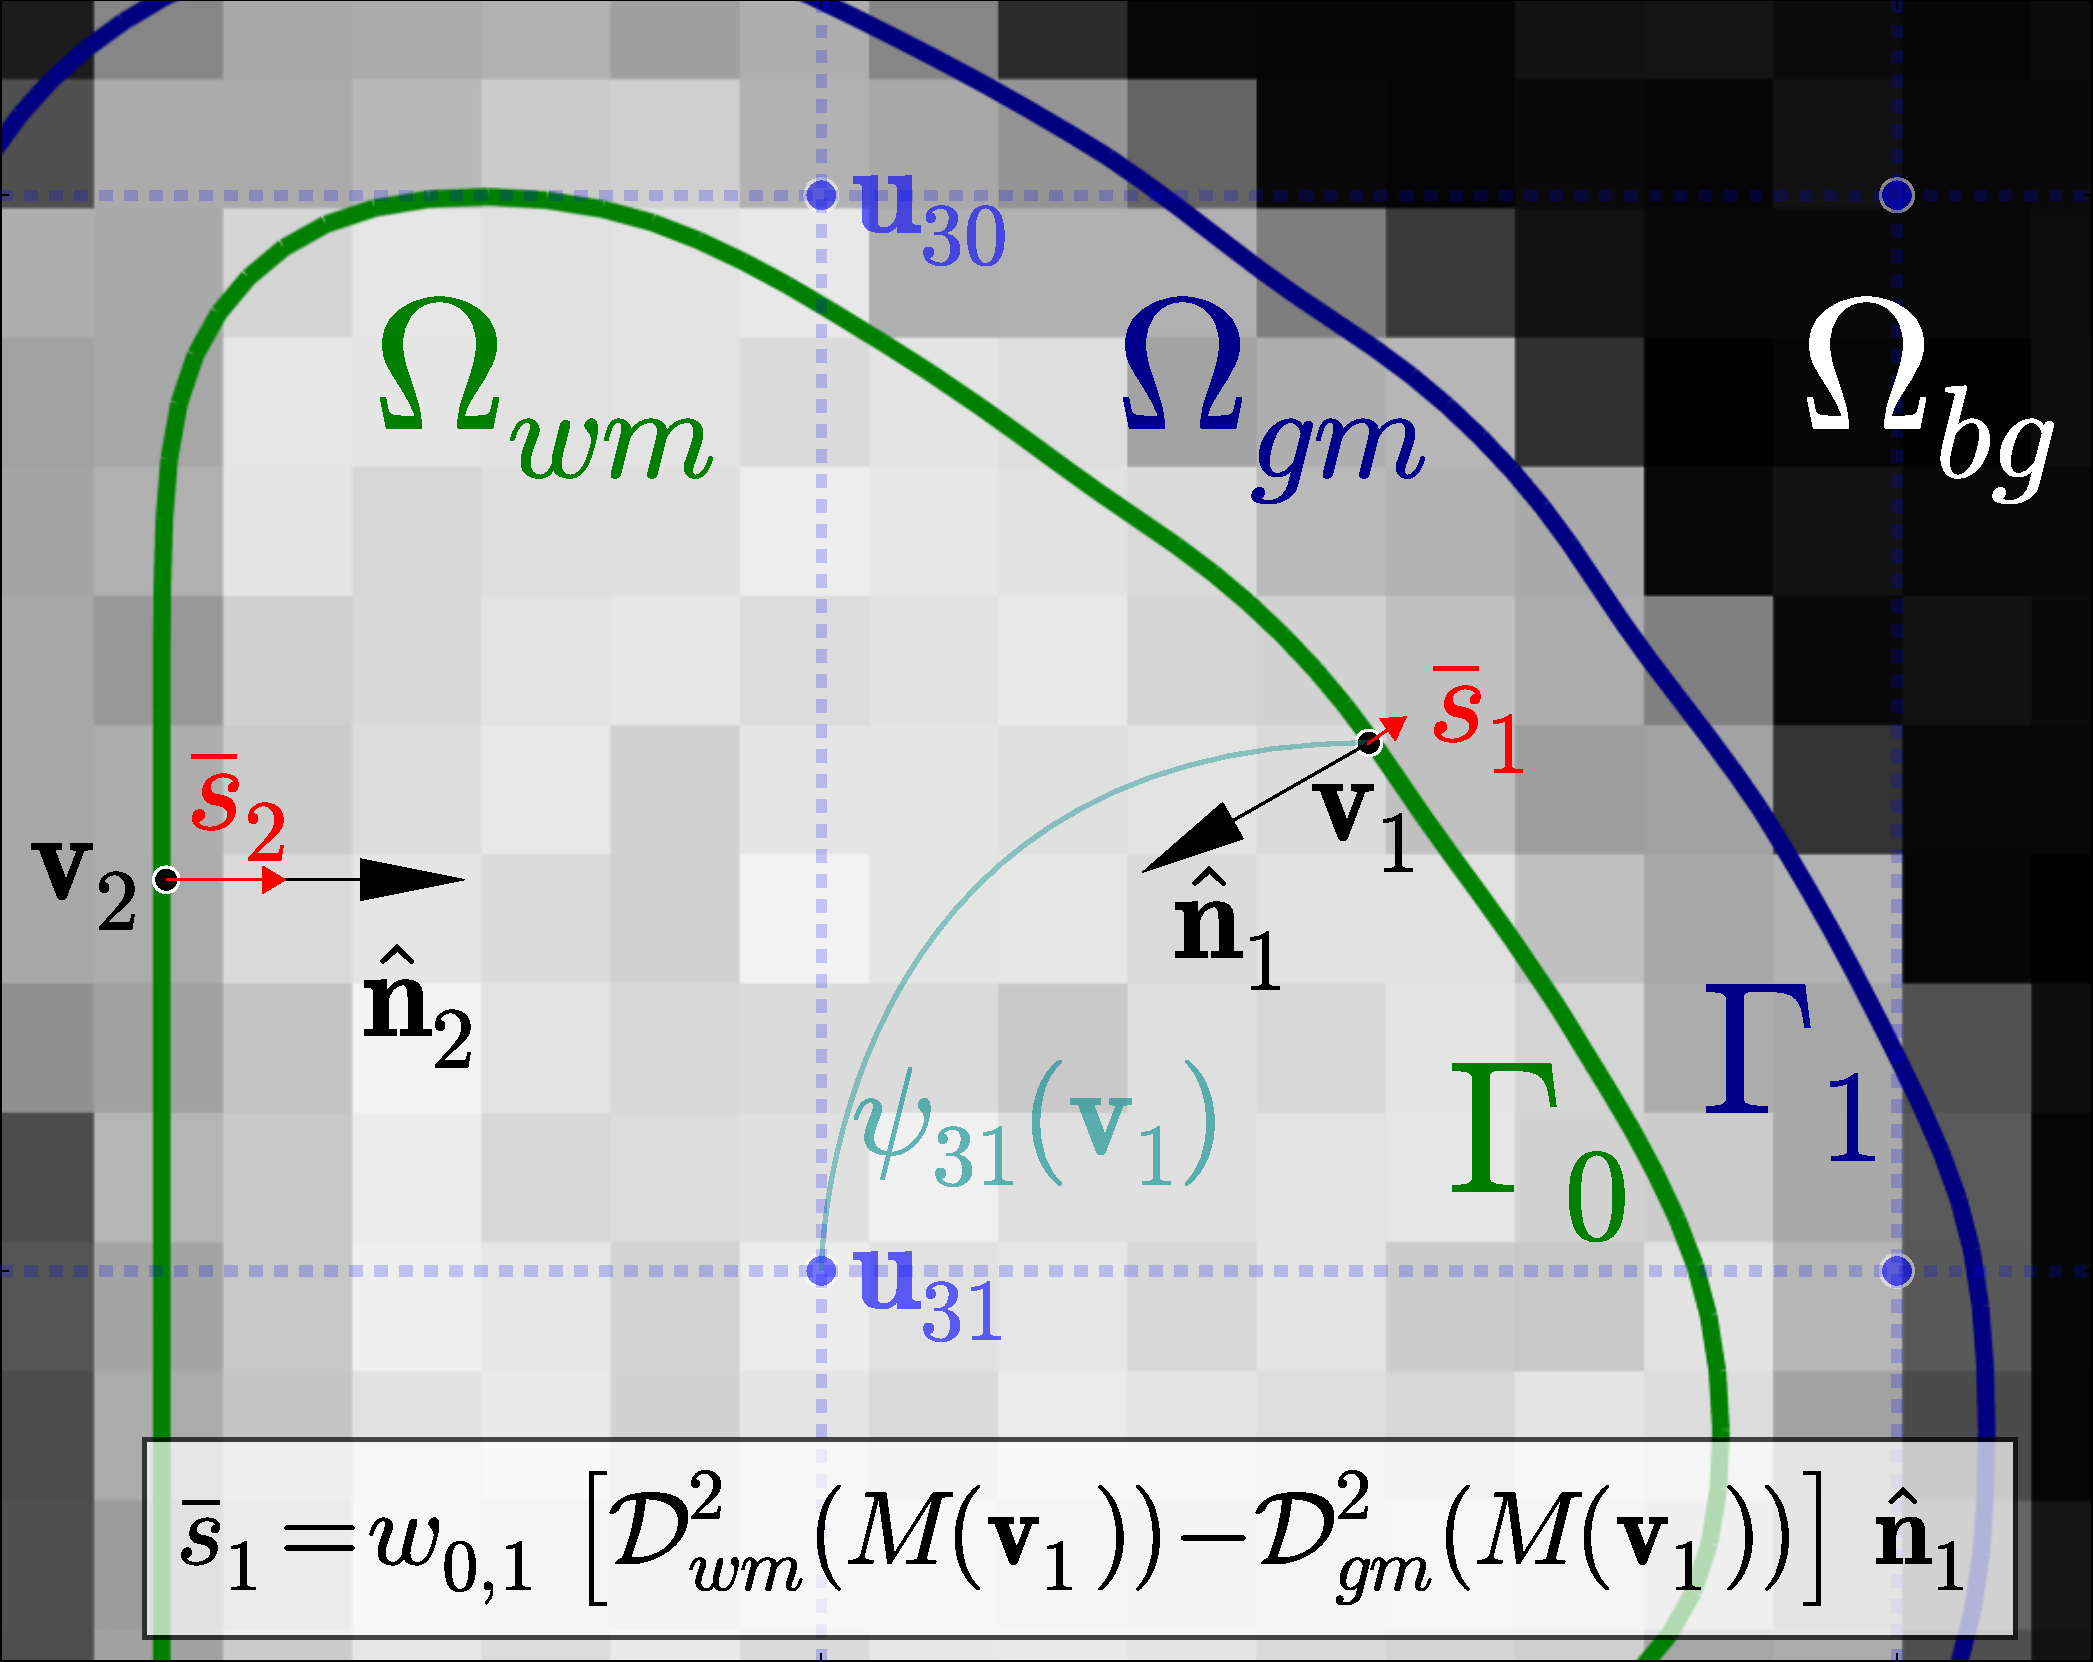
\includegraphics[width=\linewidth]{figures/figure01}
	\caption{The active contours are defined as the interfacing surfaces of the competing
	  \glspl{roi} $\Omega_i$.
	They are represented in green and dark blue colors in this close-up.
	They iteratively evolve following their inner normals $\hat{n}_i$ at each vertex
	  $\vec{v}_i$ of the mesh.
	The gradient speeds $\bar{s}_i$ are computed as the disparity between data energies of
	  the vertex $\vec{v}_i$ in each limiting region (see \ref{app:shape_priors}).
	In this figure, the gradient speed corresponding to $\vec{v}_1$ is written in the lower
	  box, $\Omega_{wm}$ being the inner limiting region and $\Omega_{gm}$ the outer.
	Finally, every $\bar{s}_i$ is associated with the control points $\vec{u}_k$ through
	  the corresponding weights $\psi_k(\vec{v}_i)$ by Eq. \eqref{eq:gradient_wshape}.
	}\label{fig:method}
\end{figure}

\paragraph*{Deformation model}\label{sec:deformation_model}
Let us denote $\{\vec{v}_i\}_{i=1 \ldots N_c}$ the vertices of one or several prior
  surface(s).
In our application, these surfaces are triangularized meshes extracted using \emph{FreeSurfer}
  \citep{fischl_freesurfer_2012}.
The transform $\hat{U}$ \eqref{eq:transform} is supported by a dense deformation field
  $\vec{u} = u(\vec{r})$, such that:

  \begin{equation}
  \vec{v}_i' = \hat{U}\{\vec{v}_i\} = \vec{v}_i + u(\vec{v}_i) = \vec{v}_i + \vec{u}_i.
  \label{eq:nodes_tfm}
  \end{equation}

Since the nodes of the anatomical surfaces likely lay off-grid, it is required to
  derive $u(\vec{r})$ from a discrete set of parameters $\{\vec{u}_k\}_{k=1 \ldots K}$.
Densification is achieved through a set of associated basis functions $\psi_k$:

  \begin{equation}
  u(\vec{r}) = \sum_k \psi_k(\vec{r}) \vec{u}_k.
  \label{eq:intp_kernel}
  \end{equation}

In our implementation, $\psi_k$ is chosen to be a tensor-product B-Spline kernel
  of degree 3 ($\beta_3$).
Then, introducing \eqref{eq:intp_kernel} into \eqref{eq:nodes_tfm} and replacing
  $\psi$ by the actual kernel function, the transformation writes:

  \begin{equation}
    \vec{v}_i' = \vec{v}_i + \sum_k \left[ \vec{u}_k \, \underset{d}{\prod}
      \beta_3( (\vec{v}_i - \vec{r}_k) \cdot \hat{\mathbf{e}}_d ) \right],
  \label{eq:transformation}
  \end{equation}
%
  with $\hat{\mathbf{e}}_d$ being the unitary vector along axis $d$.


\paragraph*{Optimization}
\label{sec:gradient_descent}
To find the minimum of the energy functional \eqref{eq:energy},
  we propose a gradient-descent approach with respect to the underlying
  deformation field through the following \gls*{pde}:

  \begin{equation}
  \frac{\partial u(\vec{r},t)}{\partial t} \propto - \frac{\partial E(R \mid U)}{\partial \vec{u}_k},
  \label{eq:general_gradient_descent}
  \end{equation}
%
  with $t$ being an artificial time parameter of the contour
  evolution, and $\vec{u}_k$ the parameters supporting the estimate
  $\hat{U}$ of the transformation at the current time point.
Now, we introduce \eqref{eq:energy} in \eqref{eq:general_gradient_descent}:

  \begin{align}
  \frac{\partial E(\vec{u})}{\partial \vec{u}_k} &=
  \frac{ \partial }{\partial \vec{u}_k} \Big\{
  \int_{\Omega} \underset{l}{\sum} \mdist{f'}{l} \,d\vec{r} \notag\\
  &+ \int_{\Omega} [ \boldsymbol{\alpha} \cdot \vec{u}^{\circ2}
  + \boldsymbol{\beta} \cdot (\nabla \vec{u})^{\circ2} ] \,d\vec{r}
  \Big\}.
  \label{eq:gradient_descent}
  \end{align}


We apply a discretized interpretation of \eqref{eq:shape_gradients} to compute
  the data term in \eqref{eq:gradient_descent} using shape-gradients
  \citep{herbulot_segmentation_2006}, and ultimately avoid level sets.
We refer the reader to the appendix \autoref{app:shape_priors} in order to fill in the gap
  between \eqref{eq:gradient_descent} and the following expression:

  \begin{align}
  \frac{\partial E_{data}(\vec{u})}{\partial \vec{u}_k} &=
  \frac{ \partial }{\partial \vec{u}_k} \left\{
   \underset{\vec{x} \in \Omega_l}{\sum} \underset{l}{\sum} \mdist{f'}{l} \right\} \notag\\
  &= \underset{i}{\sum} w_i
   \left\langle \frac{\partial \vec{v}_i'}{\partial \vec{u}_k}, \bar{s}_i'\right\rangle,
  \label{eq:gradient_wshape}
  \end{align}
%
  in this case, the formulation has been adapted to the non-binary case, $\{l,m\}$
    being any pair of neighboring regions, and $\Gamma_{l,m}$ the contour separating
    them such that
    $\vec{x}' = \vec{v}' \in\Gamma_{l,m} \iff \vec{x}\in \partial\Omega_i \cap \partial\Omega_j$,
    $\bar{s}_i'$ is the speed vector projected on to the unit inward normal to the contour
    at $c_i'$ (described in \autoref{fig:method}), $w_i$ is the area contribution of vertex
    $c_i'$ to the the total area of the surface it belongs.


Finally, we can compute:

  \begin{align}
  \frac{\partial \vec{v}_i'}{\partial \vec{u}_k} &= \frac{\partial}{\partial \vec{u}_k}
  \left\{ \vec{v}_i + \sum_k \psi_k(\vec{v}_i) \vec{u}_k \right\}
  = \psi_k(\vec{v}_i)\, \hat{\vec{e}}
  \label{eq:basis_derivative}
  \end{align}
%
  where $\hat{\vec{e}}$ is the coordinates system's unit vector.
The vertex speeds $\bar{s}_i'$ obtained by computing the shape-gradients \eqref{eq:shape_gradients},
	are then projected to the deformation field in order to obtain the derivatives $\vec{g}_k$
	corresponding to $\vec{u}_k$:

  \begin{equation}
  \vec{g}_{i,k} = w_i \, \left\langle \frac{\partial}{\partial \vec{u}_k}{\vec{v}_i}', \bar{s}_i'\right\rangle
  = - w_i \left[ \mdist{f_i'}{l} - \mdist{f_i'}{m} \right] \psi_k(\vec{v}_i)\, \hat{\vec{n}}_i,
  \end{equation}
%
  then the full gradient evolution equation \eqref{eq:gradient_descent} yields:

  \begin{align}
  \frac{\partial E(\vec{u}_k)}{\partial \vec{u}_k} =
  &\underset{i}{\sum} \vec{g}_{i,k} +2\, \boldsymbol{\alpha} \vec{u}_k
  -2\, \boldsymbol{\beta} \Delta \vec{u}_k,
  \label{eq:gradient_final}
  \end{align}

Finally, we introduce a step size parameter $\delta$ to discretize the artificial time parameter
  in the iterative optimization.
Then, applying the Fourier transform as detailed in the \suppl{section S1}, the
  update equation is derived from \eqref{eq:gradient_final}:

  \begin{align}
  \vec{u}_k^{t+1} = \mathcal{F}^{-1}\left\{ \frac{\mathcal{F}\{\vec{u}_k^t / \delta - \sum_i \vec{g}_{i,k}\}}%
                  {\mathcal{F}\{(1/\delta+\boldsymbol{\alpha})I-\boldsymbol{\beta}\Delta\}} \right\}
  \label{eq:update_equation}
  \end{align}


\paragraph*{Settings, implementation details, and convergence}
\label{sec:conv_report}
The registration parameters (such as $\delta$, $\boldsymbol{\alpha}$, $\boldsymbol{\beta}$,
  the B-Spline grid resolutions, target image smoothing, etc.)
  and other implementation details (for instance the sparse matrix approach
  to fast interpolation) are discussed in the \suppl{section S1}.
The actual choices of parameter settings are publicly distributed with the source code of the experiments.
Additionally, we release our software along with a tool for generating convergence reports to
  demonstrate the behavior of \emph{regseg} and help scientists configure their own experiments.
One sample report is found in the \suppl{section S1.3}.


\subsection{Experiments and evaluation}
\label{sec:experiments_evaluation}
%
In order to demonstrate the performance of \emph{regseg}, we first conducted a battery of
  accuracy tests over synthetic data, and then applied it in the susceptibility distortion
  correction of real data.
\autoref{fig:evworkflows} presents the workflow implementing the evaluation instruments.
Besides a visual assessment of the results, we report quantitative evaluations using
  two metrics.
In the case of the phantoms, since we had produced distortions along the three
  available dimensions, we computed the Haussdorf distance, by reusing the
  ``point-to-cell'' method of \cite{commandeur_vtk_2011}.
Conversely, the susceptibility-derived distortions only happen along the \gls*{pe}
  axis of the image.
Therefore, a \gls*{swindex} can be computed as the one-to-one distance between corresponding
  vertices of surfaces, weighted by their respective Voronoi area $a_i$:

  \begin{equation}
  sWI = \frac{1}{P} \sum\limits_p^P \frac{1}{A_p} \sum\limits_i^{N_p} a_i\,\|
  \vec{v}_i - \hat{\vec{v}}_i \|
  \label{eq:swindex}
  \end{equation}
%
  where $\vec{v}_i$ are the locations of the $N_p$ vertices in each $p \in \{1, \dots P\}$
  prior, $A_p$ the total area of surface $p$, and $\hat{\vec{v}}_i$ is the location
  recovered corresponding to the vertex $\vec{v}_i$.


\begin{figure*}
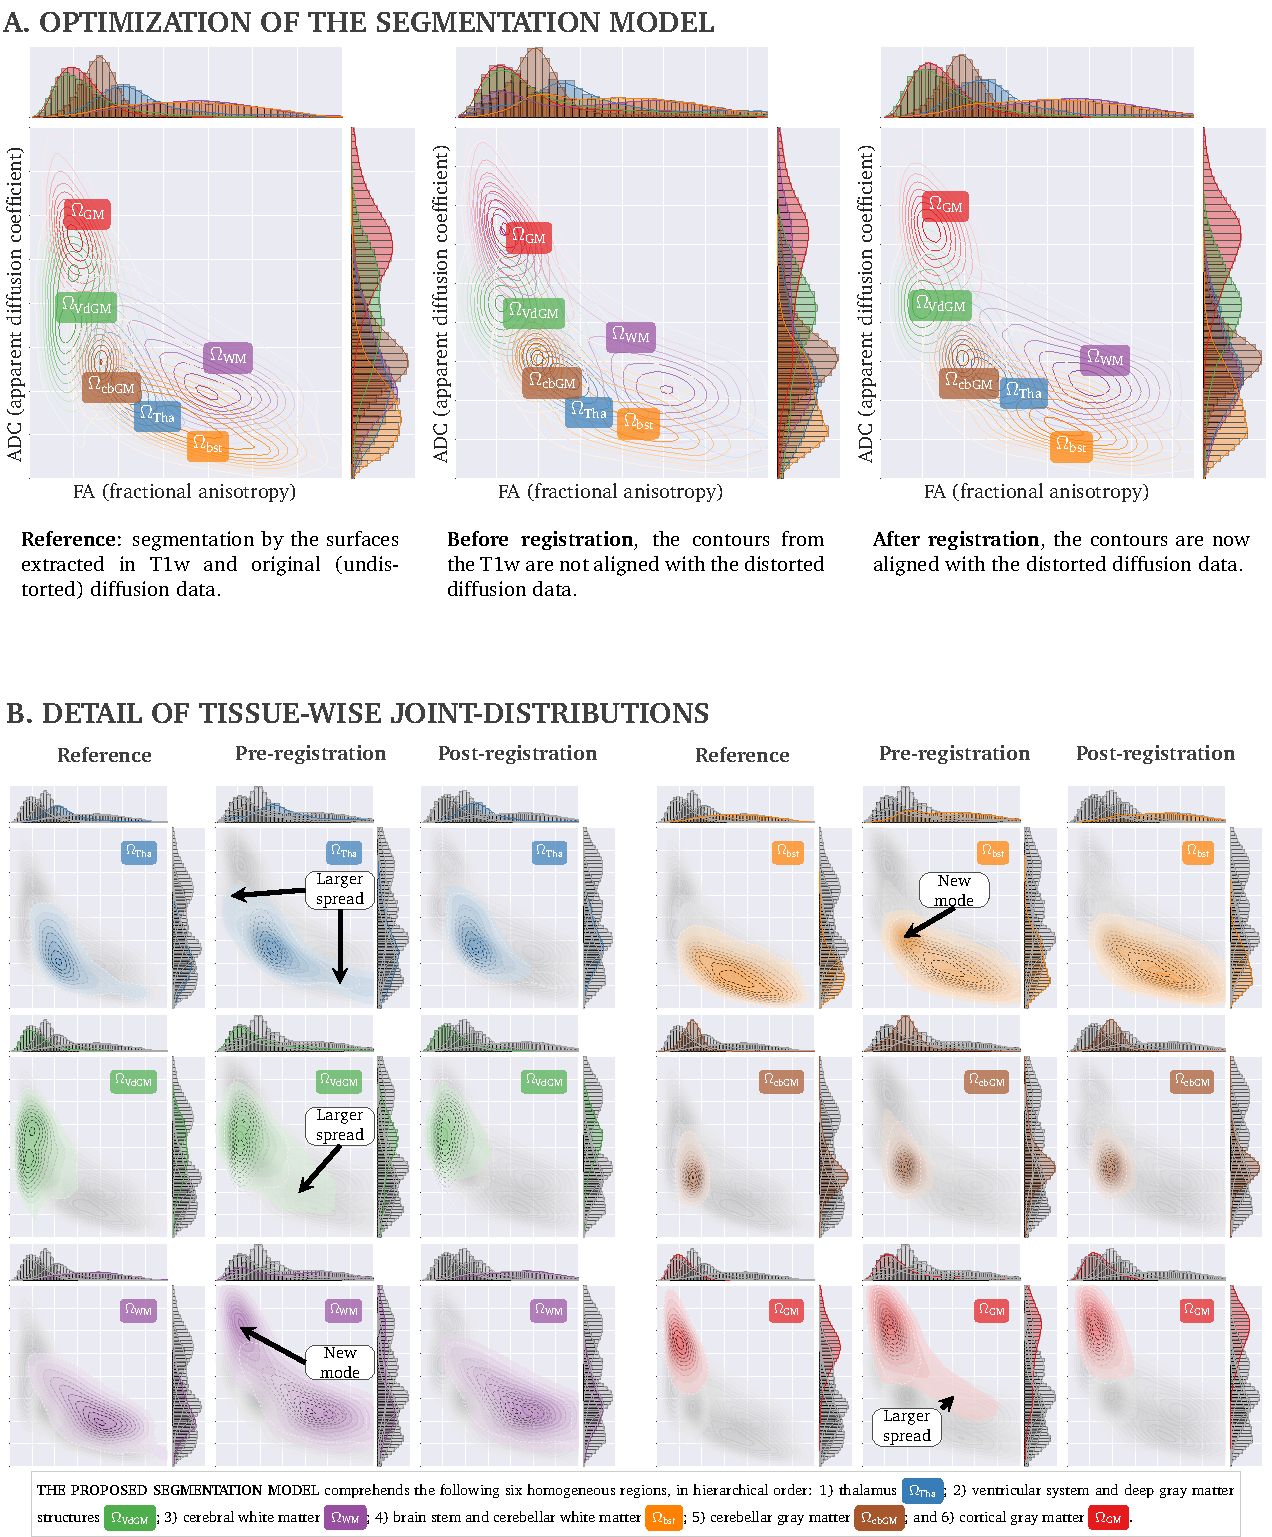
\includegraphics[width=\linewidth]{figures/figure02}
\caption{Experimental workflow applied on real data from the \acrfull*{hcp}.
  1) The prior surfaces are extracted from the anatomical reference (\gls*{t1} image).
	2) To operate as ground truth, we generate a plausible-synthetic distortion $U_{true}$
	  from the fieldmap using \eqref{eq:fieldmap}.
	3) The \gls*{dmri} data are warped using $U^{-1}_{true}$ to reproduce the effects of real
	  susceptibility-derived distortions.
	Target diffusion scalars (\gls*{fa} and \gls*{adc}) are computed on the distorted data and
		stacked to feed the multivariate input required by our algorithm.
	4) \emph{Regseg} is run, obtaining a $U_{test} = \hat{U}_{true}$, the estimation of
	  the ground-truth deformation.
	5) Results are visually and quantitatively evaluated.}\label{fig:evworkflows}
\end{figure*}


\subsection{Image Data and preprocessing}
\label{sec:datasets}

\paragraph*{Simulated phantoms}%
\label{sec:digital_phantoms}
We proved the concept on simplistic digital phantoms which we will name after their
  appearance as ``box'', ``ball'', ``L-shape'', and ``gyrus'' (\autoref{fig:phantom},
  boxes A and B).
Using \emph{phantomas} \citep{caruyer_phantomas_2014}, we simulated
  \gls*{t1} (TE/TR=10/1500ms) and \gls*{t2} images (TE/TR=90/5000ms)
  corresponding to each phantom type, with two resolutions each
  ($1.0mm$ and $2.0mm$ isotropic).
Simulations were corrupted with rician noise for a \gls*{snr} of 300.0.
The reference surfaces were extracted at the higher resolution (1.0mm isotropic),
  using \texttt{mri\_tessellate}\footnote{A marching-cubes algorithm shipped with 
  \emph{FreeSurfer} \citep{fischl_freesurfer_2012}}.

\begin{figure*}
	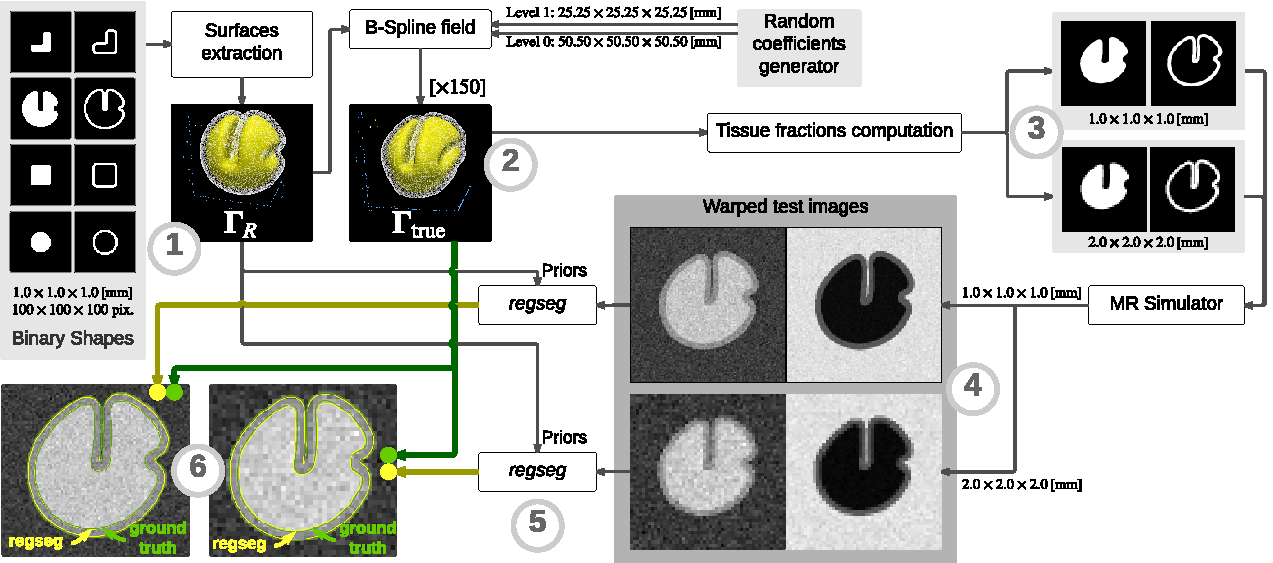
\includegraphics[width=\linewidth]{figures/figure03}
	\caption{A. The ``cortex'' phantom is a spherical shape with two sulci and an
	  outer crust resembling the cortical folding (left).
	The model is used to generate \gls*{t1} and \gls*{t2} images after warping the
	  contours using a random and plausible transformation $U_{true}^{-1}$ (right).
	B. Visual assessment of the results on the low resolution sets:
	  ``gyrus'' (top-left), ``L-shape'' (top-right), ``ball'' (bottom-left),
	  and ``box'' at (bottom-right).
	In yellow color, the recovered contours after registration are represented.
	Our method showed high accuracy, as demonstrates almost exact location of the registered
    contours with respect to their ground truth position depicted in green.
	Partial volume effect turns segmentation of the sulci a challenging problem with voxel-wise
	  clustering methods, but it is successfully segmented with our method.
	C. Quantitative evaluation of registration error in terms of average Hausdorff distance of
	  surfaces at high (left) and low (right) resolutions, demonstrating that the error is
	  consistently below the voxel size.
	  }\label{fig:phantom}
\end{figure*}

To warp the simulated datasets, we generated 150 different realizations of
  the distortion $U_{true}$.
Smoothness is introduced using two levels of B-Spline functions, with control points evenly
  located in isotropic grids covering the full extent of the phantom.
The first level had $50.5mm$ of separation between control points and the second $25.25mm$.
The rationale behind this choice is producing large deformations on the contours with
  the first level, and matching the properties of susceptibility-derived distortions
  as previously reported by \cite{irfanoglu_susceptibility_2011} with the finer grid.
The coefficients of the B-Spline functions were randomly generated for each resolution level.
Invertibility of $U_{true}$ is ensured by controlling the maximum displacement at each
  level ($20.2mm$ and $10.1mm$ respectively) as studied in \citep{rueckert_diffeomorphic_2006}.

\paragraph*{Real datasets} %
\label{sec:human_connectome}
%
For the evaluation of the algorithm on real \gls*{dmri} data of human brains,
  we collected 16 datasets from the ``minimally preprocessed''
	 database of the \gls*{hcp}.
We refer the reader to \citep{essen_human_2012} for exact details about acquisition
  parameters, and \citep{glasser_minimal_2013} for the preprocessing issues.
The datasets comprehend a large set of images, containing \gls*{t1}, \gls*{t2} and
  multi-shell \gls*{dmri} images.
The original acquisitions are released within ``unprocessed'' packages, and
  the ``minimally preprocessed'' are corrected for artifacts, brain-extracted
  and spatially normalized, along with some results of the standard processing
  pipeline of \emph{FreeSurfer}.

Selecting the appropriate labels in the \emph{aparc} segmentation, we applied
  \texttt{mri\_tessellate} to extract the surface of the following
  six homogeneous regions $\Omega_l$:
  1) the thalamus, $\Gamma_{Tha}$;
  2) \gls*{csf} of the ventricular system and deep \gls*{gm} structures, $\Gamma_{VdGM}$;
  3) cerebral \gls*{wm}, $\Gamma_{WM}$;
  4) brain stem and cerebellar \gls*{wm}, $\Gamma_{bst}$;
	5) cerebellar \gls*{gm}, $\Gamma_{cbGM}$; and
	6) cortical \gls*{gm} surface, $\Gamma_{pial}$.
The choice of this particular model is further addressed in \autoref{sec:res_model_and_metric}.

In this case, we derived the deformation $U_{true}$ from the field maps released with
  the corresponding packages of each dataset from the \gls*{hcp} applying \eqref{eq:fieldmap},
  mimicking the real distortions, using a derivation of our previous work
  \citep{esteban_simulationbased_2014}.
After warping the original \gls*{dmri} with $U_{true}^{-1}$, we computed the \gls*{dti} and
  the derived scalars (\gls*{fa} and \gls*{adc}) using \emph{MRtrix} \citep{tournier_mrtrix_2012}.
The stack of \gls*{fa} and \gls*{adc} conforms the multivariate input for \emph{regseg}.

A dual workflow to the general evaluation framework (\autoref{fig:evworkflows})
  was also implemented to integrate the \gls*{t2b} registration scheme.
We reproduced the solution and settings provided with \emph{ExploreDTI}
  \citep{leemans_exploredti_2009}, a widely used toolkit for tractography analysis of
  \gls*{dti}.
\emph{ExploreDTI}, internally uses \emph{elastix} \citep{klein_elastix_2010} to
  perform registration.
First, the average \emph{b0} volume is computed using all the \emph{low-b} volumes within
  the distorted \gls*{dmri} dataset.
Using the ``preprocessed'' instance of the \gls*{t2} image of the corresponding subject as
  reference image, and the \emph{b0} image as moving image, we registered both and
  projected the correct (undistorted) contours to the warped space using the resulting
  transform.

\section{Data and experiments}
\label{sec:experiments}
%
\subsection{Shape prior}
%
As described in \autoref{sec:introduction}, the general situation in
the connectivity pipelines consists of having 
a reliable segmentation obtained from the high resolution \gls{t1} 
reference image. Therefore, a precise location of the tissue interfaces
of interest is available in a reference space. Given that the anatomical 
reference segmentation is beyond the scope of this manuscript, we simply 
rely on the true contours known from the underlying models, and do not 
seek to establish them in a separate segmentation step on ``anatomical'' images.
%
\subsection{Synthetic gray-scale data}
%
The first simplified model to test the approach is inspired by a problem 
shown for coupled \gls{csf}/\gls{gm} and \gls{gm}/\gls{wm} segmentation in \citep{macdonald_automated_2000}. Authors note that ``partial volume effects 
blur the distinction between closely adjacent surfaces in deep sulci, leading 
to a well-known segmentation error in which the deeper reaches of sulci are 
not penetrated by the putative surface model.'' This problem is aggravated 
in DWI, since the resolution tends to be worse compared to the anatomical 
images considered in \citep{macdonald_automated_2000}. They test their 
coupled segmentation algorithm on an image, ``representing a sulcus in 
which the distinction between opposing banks of the sulcus has been obscured 
by partial volume.''  

Here, we reproduce their model on a volume consisting of three 
piecewise-constant parts: a notched ball representing the \gls{wm} with a single 
sulcus ($\mu_{WM} = 0.8$), a cortical sheet of \gls{gm} obtained through dilation 
of the \gls{wm} ($\mu_{GM} = 0.5$), and the surrounding background representing 
\gls{csf} ($\mu_{CSF} = 0.2$). The volume is then affected by additive Gaussian 
noise, effectively creating uniform standard deviation of $\sigma = 0.045$ per 
region.

As illustrated in \autoref{fig:sulcusmodel}, conventional single surface 
segmentation of the \gls{csf}/\gls{gm} boundary misses to capture the sulcus in 
its full depth. With our proposed model, we expect the joint 
segmentation-registration to be driven largely by the inner, \gls{gm}/\gls{wm}
contour that exhibits sufficient contrast and lesser partial volume effects. 
The shape prior of the outer, difficult contour will then be co-aligned through 
the regularity of the estimated deformation field.

\begin{figure}
\begin{tabular}{ccccc}
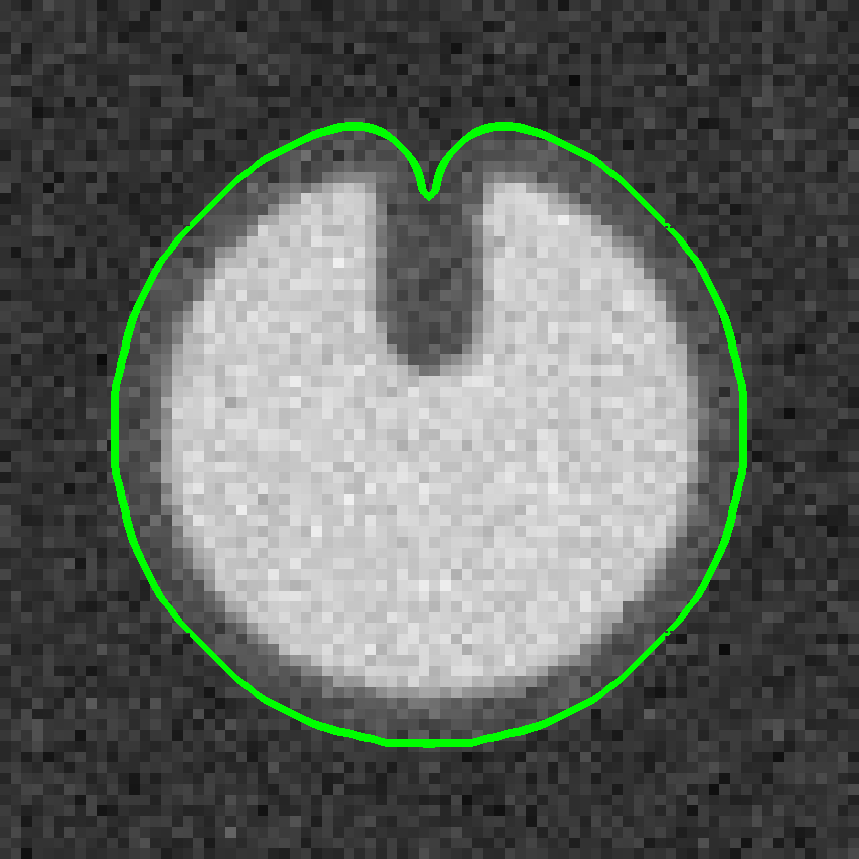
\includegraphics[width=0.19\textwidth]{contours_wrong} & 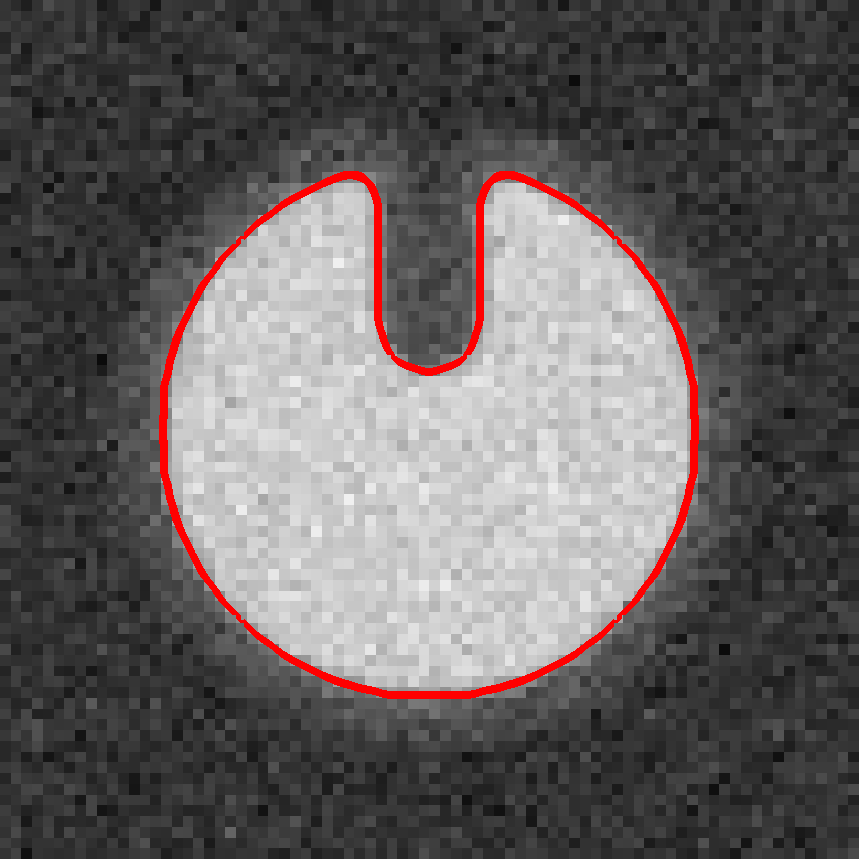
\includegraphics[width=0.19\textwidth]{contours_inner} &
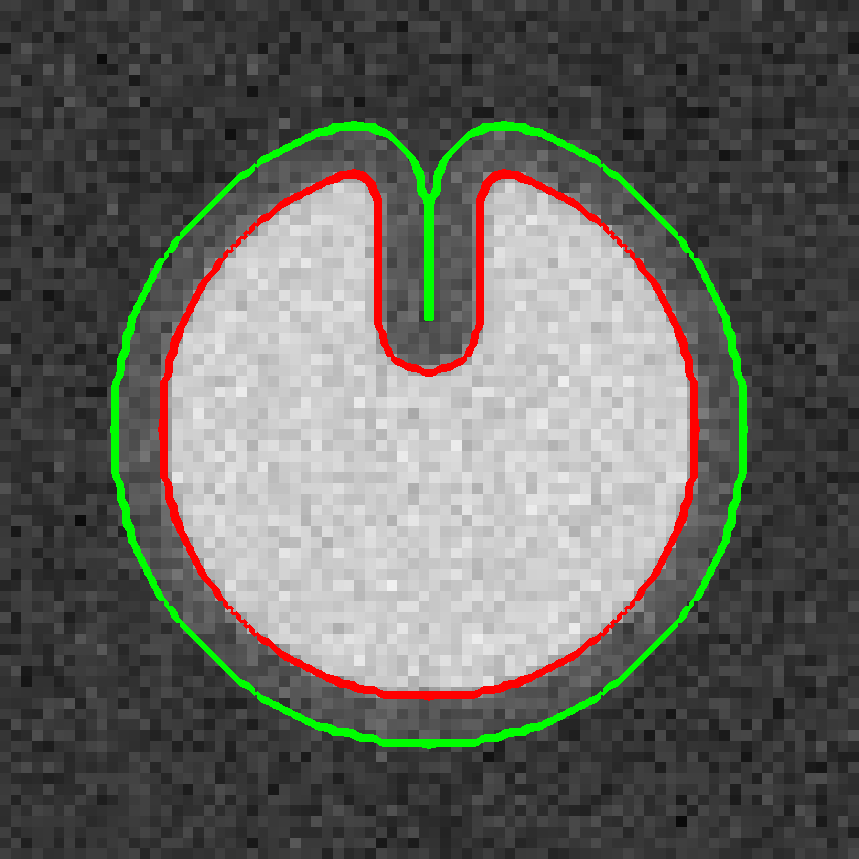
\includegraphics[width=0.19\textwidth]{contours_both} &
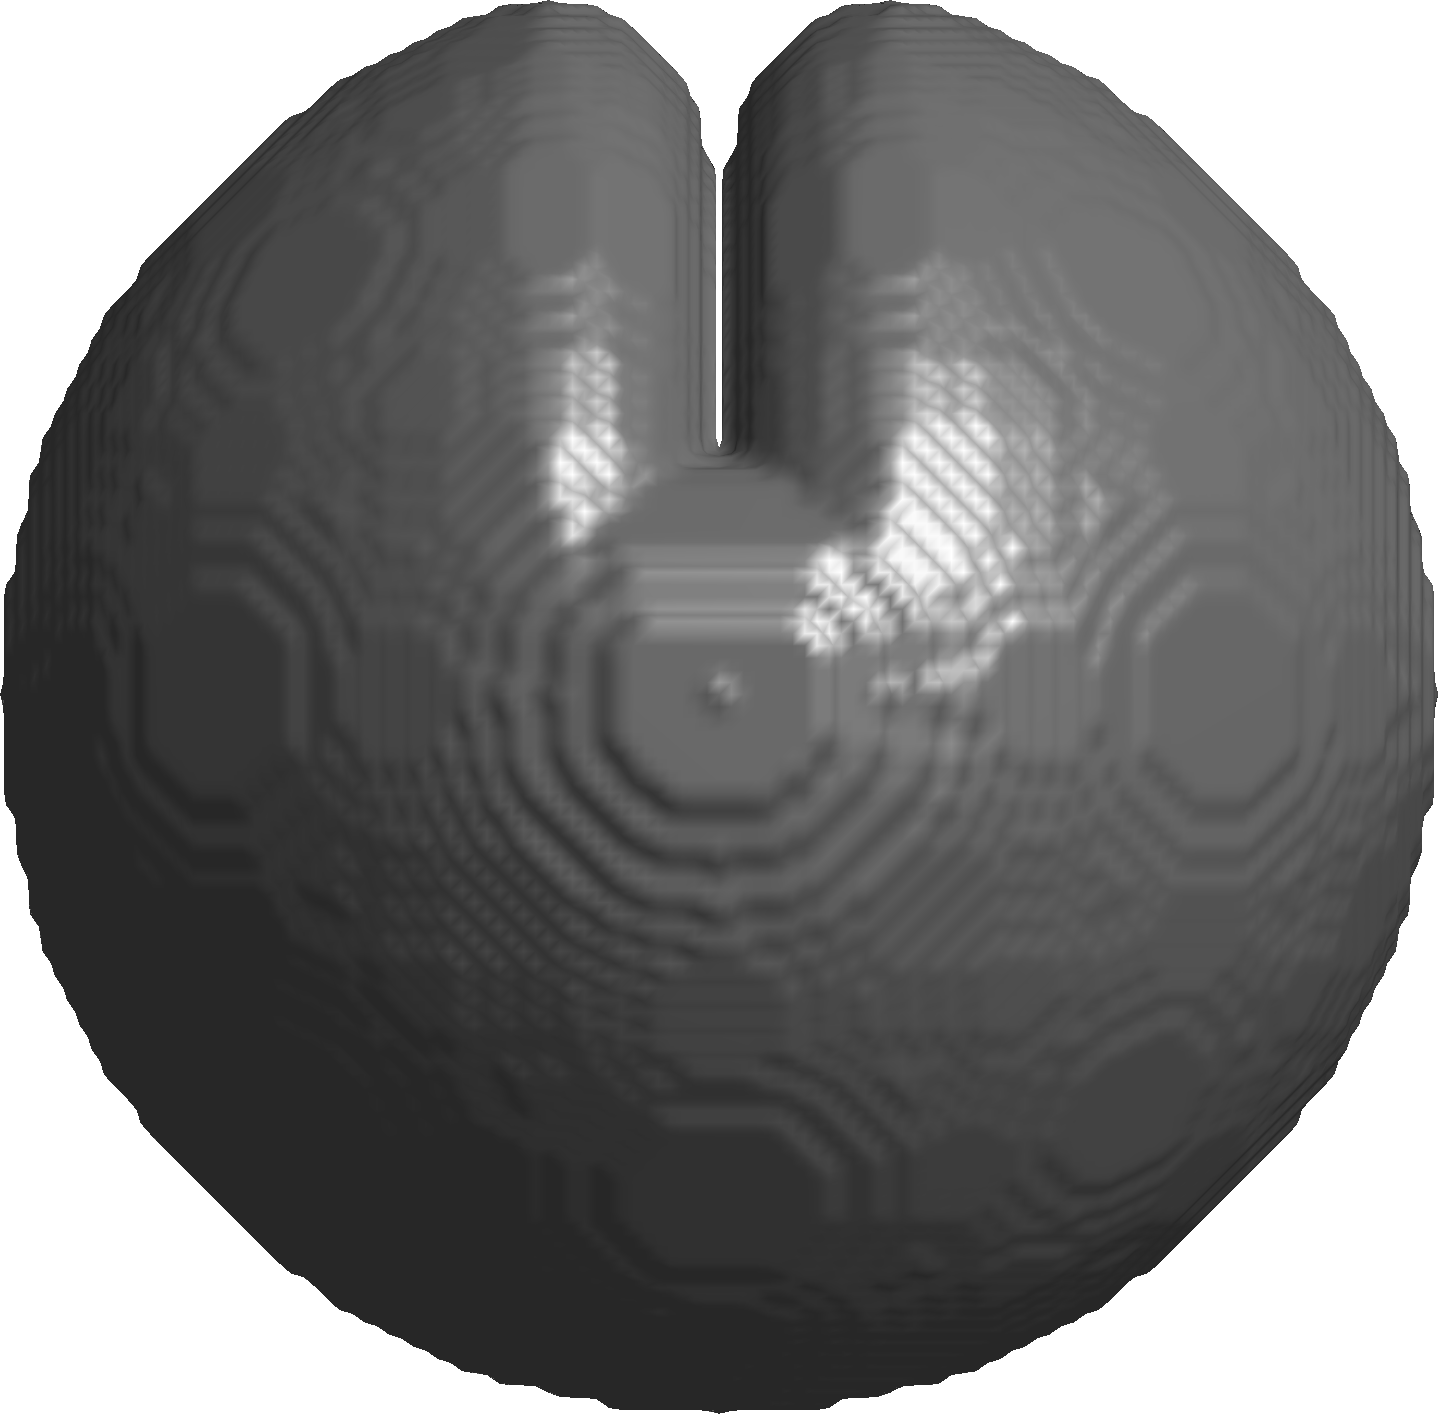
\includegraphics[width=0.19\textwidth]{pialsurf} &
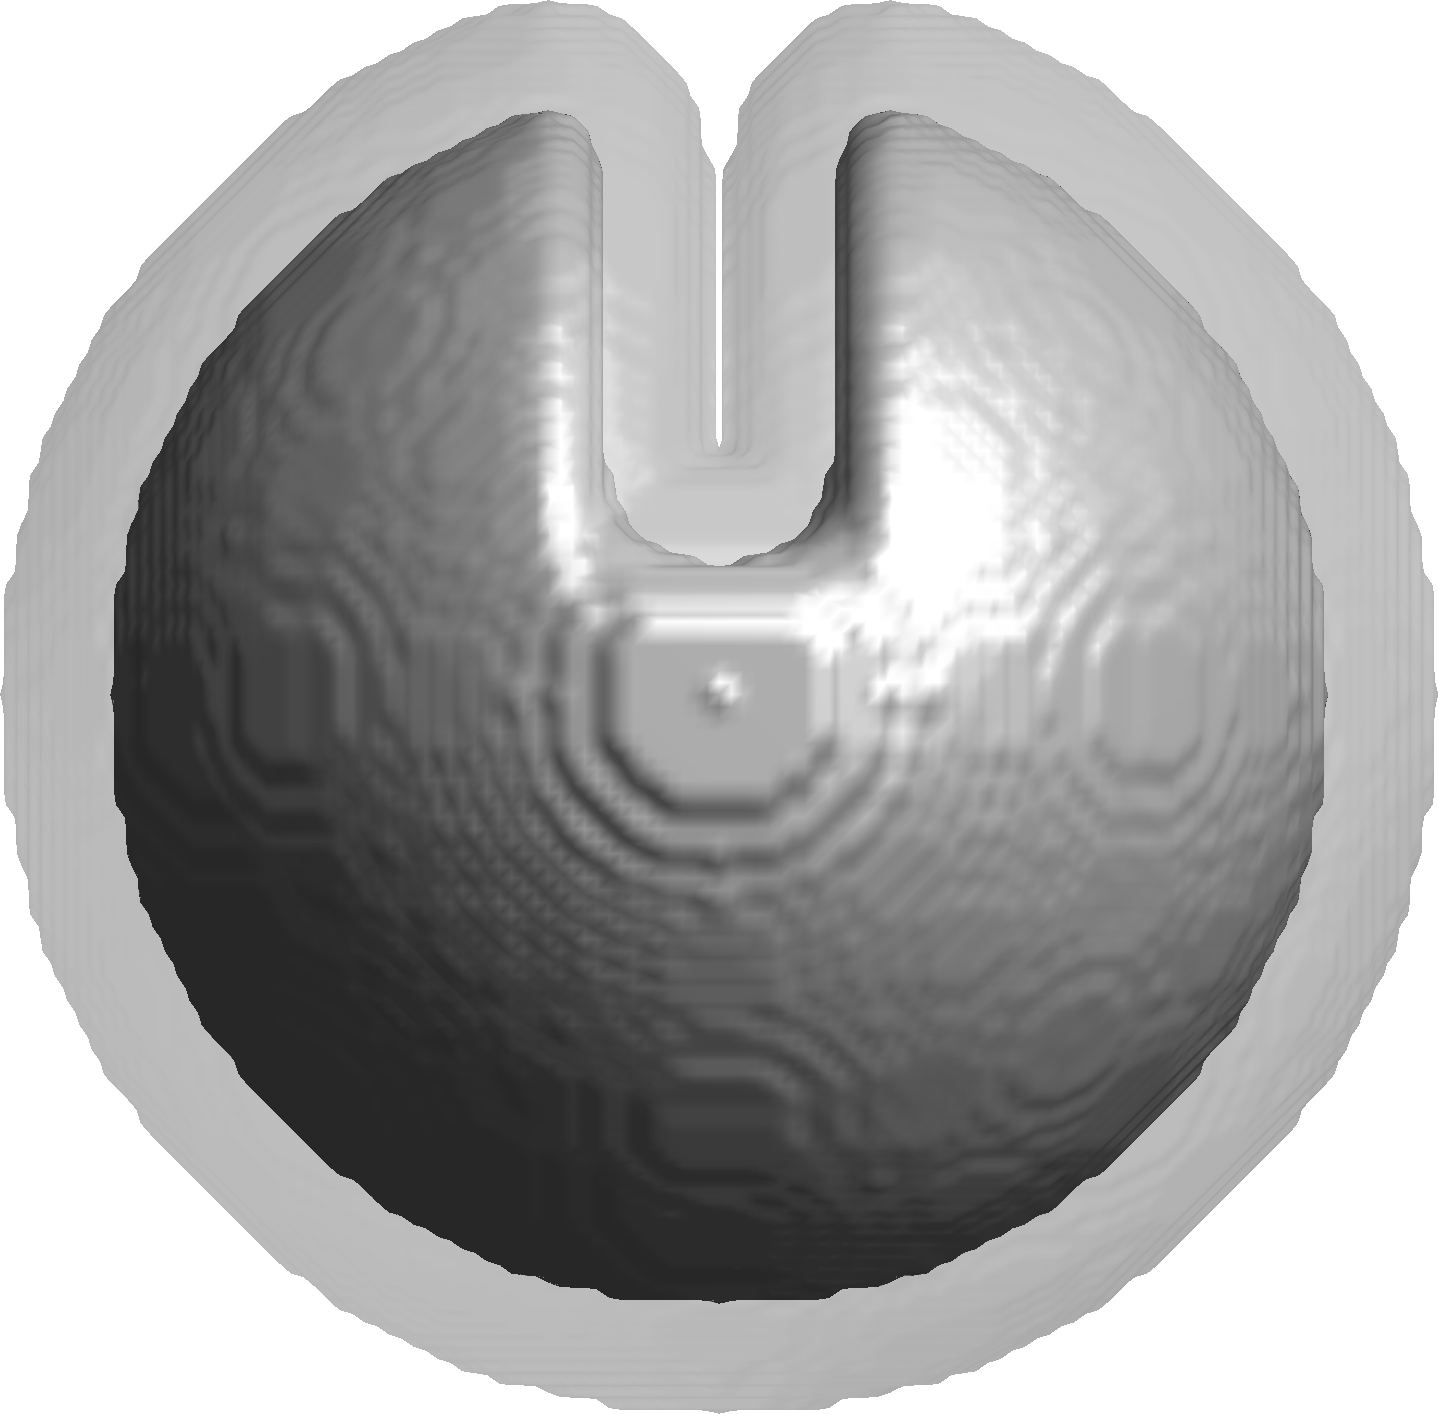
\includegraphics[width=0.19\textwidth]{gmwmsurf}\\
a)&b)&c)&d)&e)
\end{tabular}
\caption{The gray-scale sulcus model. a) The apparent CSF/GM boundary is affected by partial volume in the sulcal cavity, and conventional segmentation is likely to miss it. b) The GM/WM interface here has consistently good contrast. c) Registering the two shape priors coupled through deformation field regularity is expected to guide the CSF/GM contour. d\&e) 3D view of the two shape priors.}
\label{fig:sulcusmodel}
\end{figure}



%
\subsection{Simulated diffusion data}
%
In order to demonstrate the functionality of the methodology, 
and characterize its possibilities with diffusion data,
we built a synthetic phantom from a model consisting of several 
spherical shapes emulating the different brain tissues (see 
\autoref{fig:fa}, first row). We simulated a single-shell
acquisition at $b=1000$ \eqref{eqn:MultiTensor} with 30 samples
equally distributed on one hemisphere, corresponding to a standard
\gls{dti} acquisition commonly used in clinical practice.
We generated a synthetic displacement field to produce
an \gls{epi}-like distortion on the \gls{dwi} signal. Finally,
we reconstructed the deformed signal, and generated \gls{dwi}-derived
scalar maps (specifically the \gls{fa} and \gls{md} maps).
Then, the scalar maps were placed as features in 
\eqref{eq:complete_energy} to drive our segmentation approach, 
finding the location of the \gls{wm}-\gls{gm}
and the \gls{csf}-\gls{wm} interfaces in the distorted space. \\

\paragraph{Signal simulation}
To numerically simulate the \gls{mri} signal attenuation when applying a diffusion 
gradient in a voxel with $N$ fiber populations we made use of the standard 
\emph{Multi-Tensor Model}~\cite{Tuch:2002aa}:
%
\begin{equation} 
\label{eqn:MultiTensor}
S(q) / S_{0} = \sum_{i=1}^{N} f_{i} \, \exp{ \left( -b \, q^{T} \, \mathbf{D}_i \, q\right) } + f_{iso} \, \exp{ \left( -b \, \mathbf{D}_{iso} \right) }  + f_{gm} \, \exp{ \left( -b \, \mathbf{D}_{gm} \right) } ,
\end{equation}
%
where $q \in \mathbb{S}^2$ is the direction of the diffusion gradient applied,
$b$ is the b-value accounting for its strength and $S_0 \equiv S(0)$ is the 
signal with no diffusion weighting. $f_i$ and $\mathbf{D}_i$ are the volume 
fraction and the diffusion tensor characterizing the $i$-th fiber population, 
whereas the tensors $\mathbf{D}_{iso}$ and $\mathbf{D}_{gm}$ describe the 
diffusion processes of partial volumes with \gls{csf} and \gls{gm} within the 
voxel, which volume fractions are, respectively, $f_{iso}$ and $f_{gm}$, and
$\sum_i f_i + f_{iso} + f_{gm} = 1$. In this work, the diffusion properties have
been taken from standard ranges typically observed in the human 
brain~\cite{Canales-Rodriguez:2009aa}. Moreover we assumed $N = 1$ and $S_0 = 1$ 
without loss of generality.

\paragraph{Noise simulation}
The diffusion MRI signal $S$ has been corrupted with 
\textit{Rician noise}~\cite{Gudbjartsson:1995aa} as follows:
%
\begin{equation}
	\tilde{S} = \sqrt{ (S + \varepsilon_1)^2 + \varepsilon_2^2 }
\end{equation}
%
where $\varepsilon_{1,2}$ are Gaussian distributed with zero mean
and standard deviation $\sigma = S_0 / \mathit{SNR}$ and \gls{snr}
is the \gls{snr} on the $S_0$ image.

\paragraph{Simulated \gls{epi} distortion}
For this model, we created manually a sound distortion to approximate
the real \gls{epi} distortions. We interpolated the distortion to a 
dense deformation field, and applied it to generate the deformed \gls{dwi}
signal.

\paragraph{Derived scalar features}
We obtained the local fiber configuration in each voxel with a commonly 
used \gls{dti} reconstruction tool~\footnote{DTIFIT, included
in the FMRIB's Software Library (FSL), 
\url{http://fsl.fmrib.ox.ac.uk/fsl/fsl-4.1.9/fdt/fdt_dtifit.html}}. 
The properties of the reconstructed tensors and derived scalar maps have
been studied by \cite{ennis_orthogonal_2006}. Based on their
findings, \gls{fa}~\eqref{eq:fa} and \gls{md}~\eqref{eq:md} are
considered complementary features, and therefore we selected them for the 
energy model \eqref{eq:complete_energy} in driving the 
registration-segmentation process. 
Whereas \gls{fa} informs mainly about the \emph{shape} of diffusion, 
the \gls{md} is more related to the \emph{magnitude} of the process:

\begin{align}
\mathrm{FA} &= \sqrt{ \frac{1}{2}}\,\frac{\sqrt{ (\lambda_1 - \lambda_2)^2 + (\lambda_2 - \lambda_3)^2 + (\lambda_3 - \lambda_1)^2}}{\sqrt{ {\lambda_1}^2 + {\lambda_2}^2 + {\lambda_3}^2}} \label{eq:fa} \\
\mathrm{MD} &= ( \lambda_1 + \lambda_2 + \lambda_3 ) / 3 \label{eq:md}
\end{align}
where $\lambda_i$ are the eigenvalues of the diffusion tensor 
associated with the diffusion signal $S(\vec{q})$. There exist 
two main reasons to justify their choice. 
First, they are well-understood and standardized in clinical routine.
Second, together they contain most of the information that is
usually extracted from the \gls{dwi}-derived scalar maps
\cite{ennis_orthogonal_2006}. The different region properties 
$(\mathbf{\mu}_R,\Sigma_R)$ measured for the \gls{fa} and \gls{md}
joint distribution are summarized in \autoref{table:parameters}. \\ 

\begin{table}
\caption{Model means and covariances of \gls{fa} and \gls{md} estimated 
from the reconstructed simulated \gls{dwi} images for each modeled tissue, 
\gls{wm}, \gls{gm}, and \gls{csf}. As expected, the two scalar features 
are complementary and the three tissues can well be discriminated. }
\label{table:parameters}
%\begin{tabularx}{1.0\textwidth}{c|XXX}
\begin{tabular}{*{3}{@{}p{0.2\textwidth}}@{}p{0.4\textwidth}@{}}
\toprule
% tissue        & $\mathbf{\mu}_{FA}$ & $\mathbf{\mu}_{MD}$ & $\Sigma$ \newline
        & $\mathbf{\mu}$ \\
\cmidrule(r){2-3}
Tissue& FA & MD &$\Sigma$\\
\cmidrule(r){1-1}\cmidrule(r){2-2}\cmidrule(r){3-3}\cmidrule{4-4}
\gls{wm}  & 0.778 & 6.94\e{-4} & 
   $\begin{pmatrix}
   	4.85\e{-3} & -6.90\e{-6} \\ -6.90\e{-6} & 1.03\e{-8}
   \end{pmatrix}$\vspace{2mm}\\
%
\gls{gm}  & 0.119 & 8.95\e{-4} &
   $\begin{pmatrix}
   	5.90\e{-4} & -1.43\e{-6} \\ -1.43\e{-6} & 1.04\e{-8}
   \end{pmatrix}$\vspace{2mm}
\\
%
\gls{csf} & 0.103 & 2.99\e{-3} &
   $\begin{pmatrix}
   	1.19\e{-3} & 2.22\e{-7} \\ 2.22\e{-7} & 1.56\e{-8}
   \end{pmatrix}$
\\
\bottomrule
\end{tabular}
%\end{tabularx}

\end{table}


\section{Results and discussion}
\label{sec:results}

\subsection{Synthetic gray-scale data}
The proposed method solved precisely the specific challenge
created by the model. A severe distortion of the model is
artificially created adding complexity to the problem of
partial voluming in the outer contour of the sulcus.
\autoref{fig:sulcusmodel_result} provides visual assessment
for this result. With 16x16x16 control points and an 
approximate total of 29,000 nodes contained by the two prior 
surfaces, computation time for this model was around
14 minutes in an \textit{Intel\textsuperscript{\textregistered} 
Core\textsuperscript{\texttrademark} i5 CPU M 430 @ 2.27GHz} and
4GB RAM.

\begin{figure}
\begin{tabular}{ccccc}
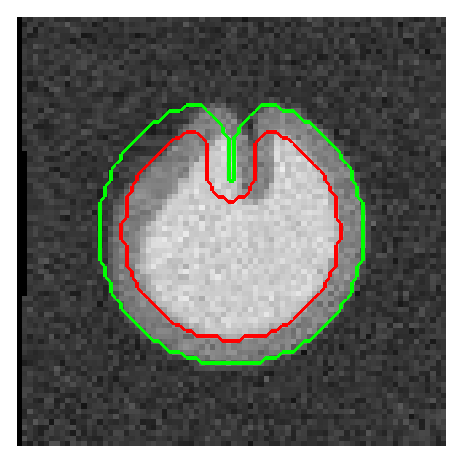
\includegraphics[width=0.19\textwidth]{model2result_b_1} &
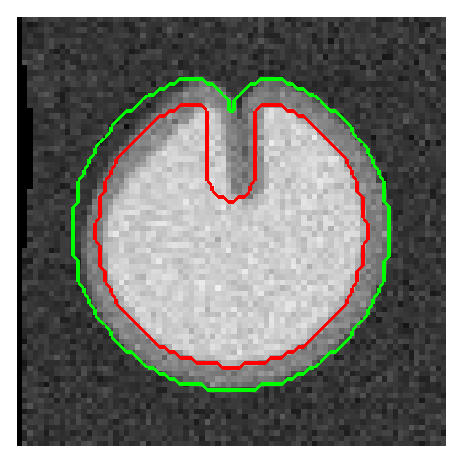
\includegraphics[width=0.19\textwidth]{model2result_b_2} &
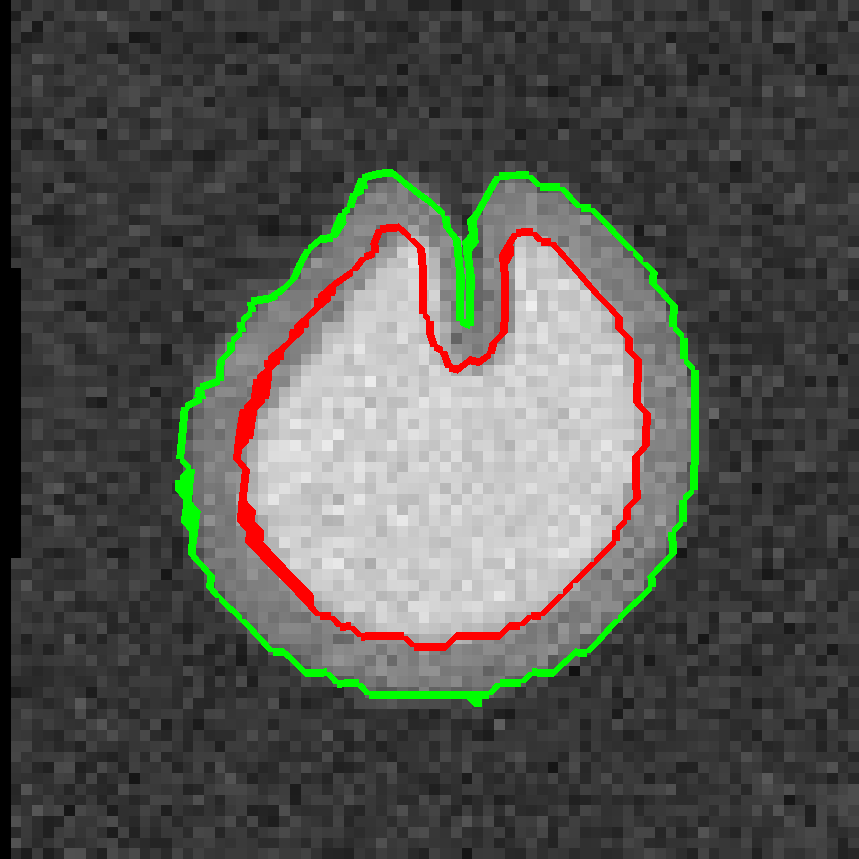
\includegraphics[width=0.19\textwidth]{model2result_a_1} &
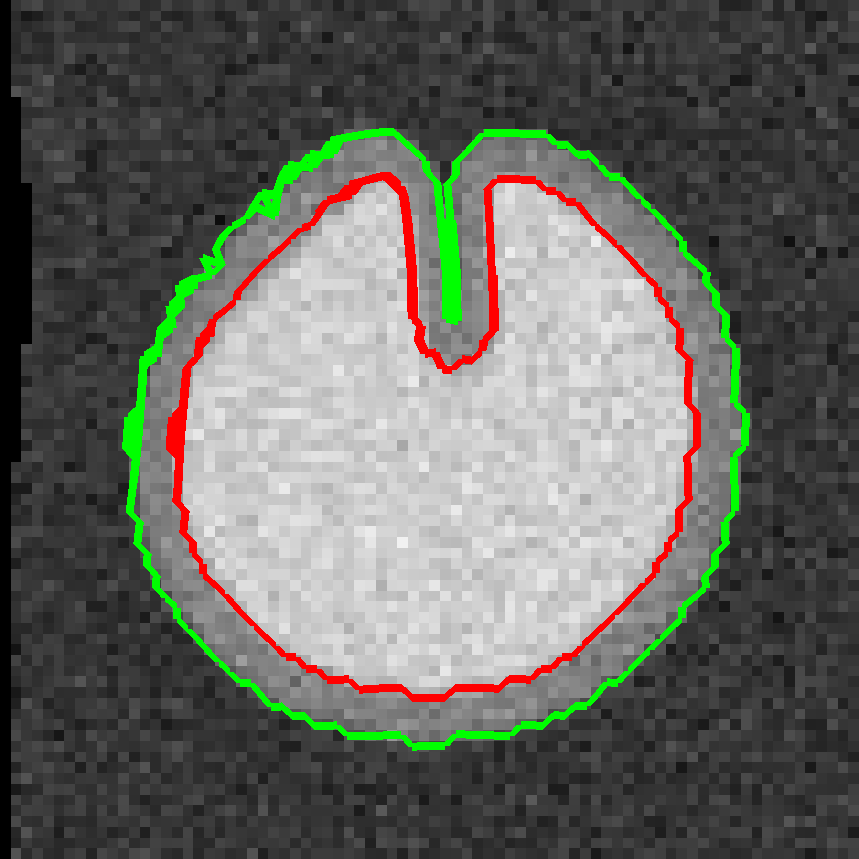
\includegraphics[width=0.19\textwidth]{model2result_a_2} &
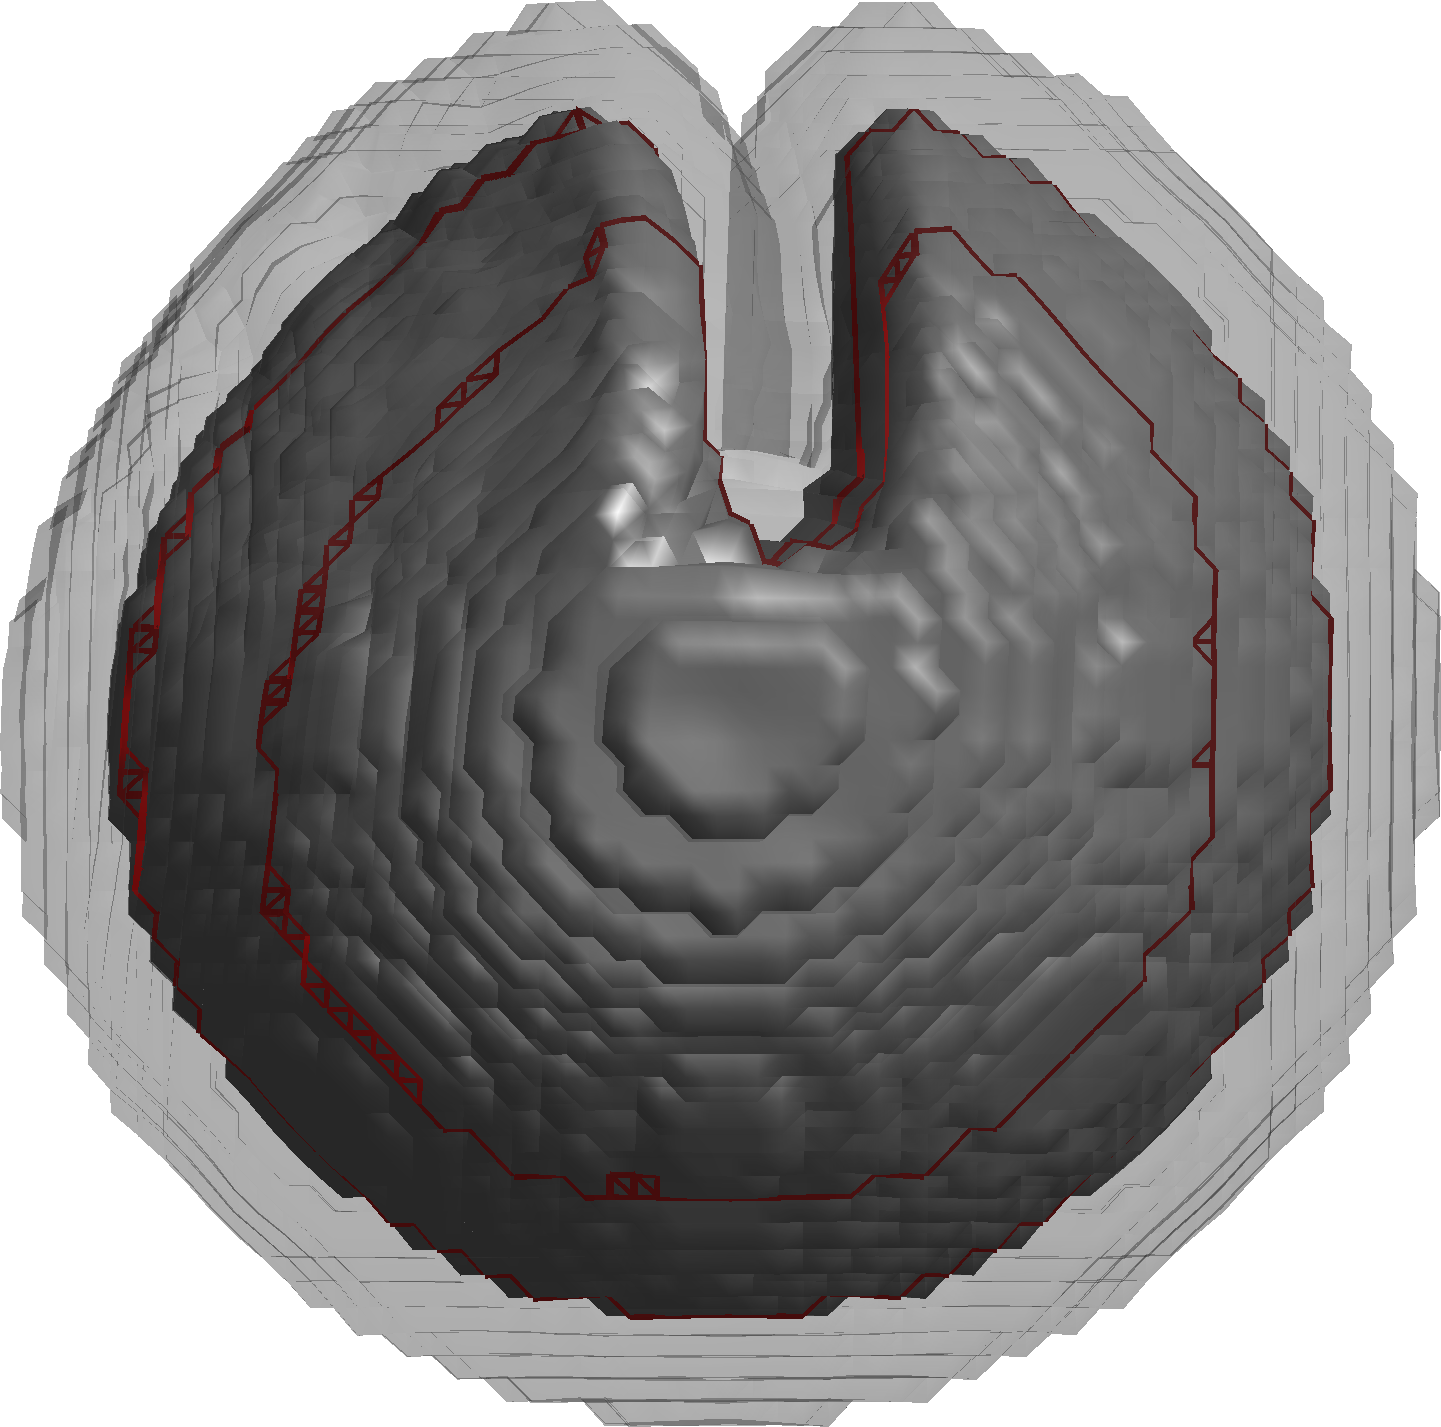
\includegraphics[width=0.19\textwidth]{model2surf} \\
\multicolumn{2}{c}{a)} & \multicolumn{2}{c}{b)} & c)
\end{tabular}
\caption{Result of the segmentation performance on the sulcus model.
a) Two slices and prior contours before segmentation-registration. b) The same slices and contours after distortion estimation. c) 3D rendering of the deformed priors, with the traces of the two selected slices highlighted.}
\label{fig:sulcusmodel_result}
\end{figure}


\subsection{Simulated diffusion data}
\label{sec:simulated_dwi}
%
The proposed method successfully reverted the synthetic distortion
field we applied to the data. Second row in \autoref{fig:fa} shows 
the fitted contours obtained by using the original surfaces of the model
as shape priors, with a constant translation of [5.0,10.0,-5.0] mm.
to illustrate briefly the extent of the capture range of the algorithm.
Computation time in this case was around 10 minutes in the previously
described platform, with 16x16x16 control points on
the dense deformation field and approximately 26,000 nodes in 
total for both prior surfaces. \\
%

%\begin{figure}
%\begin{tabular}{ccccc}
%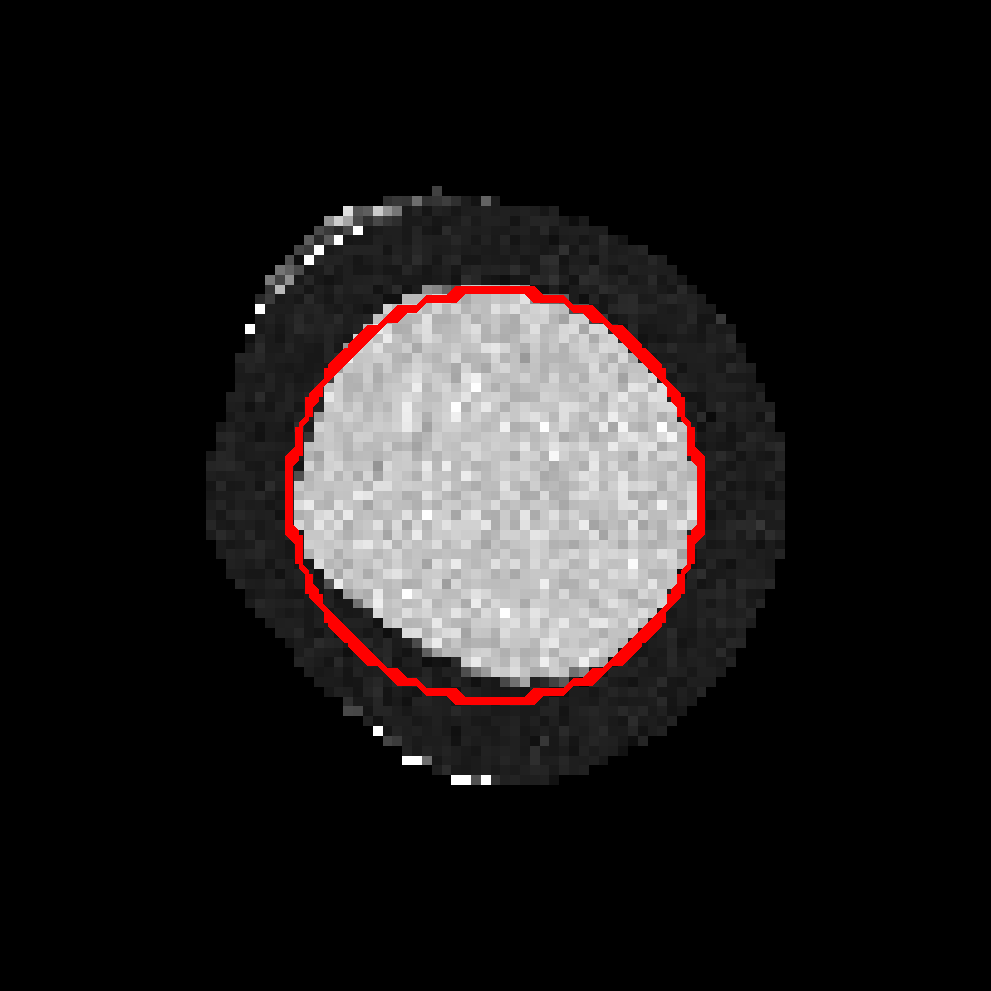
\includegraphics[width=0.19\textwidth]{model1result_b_1} &
%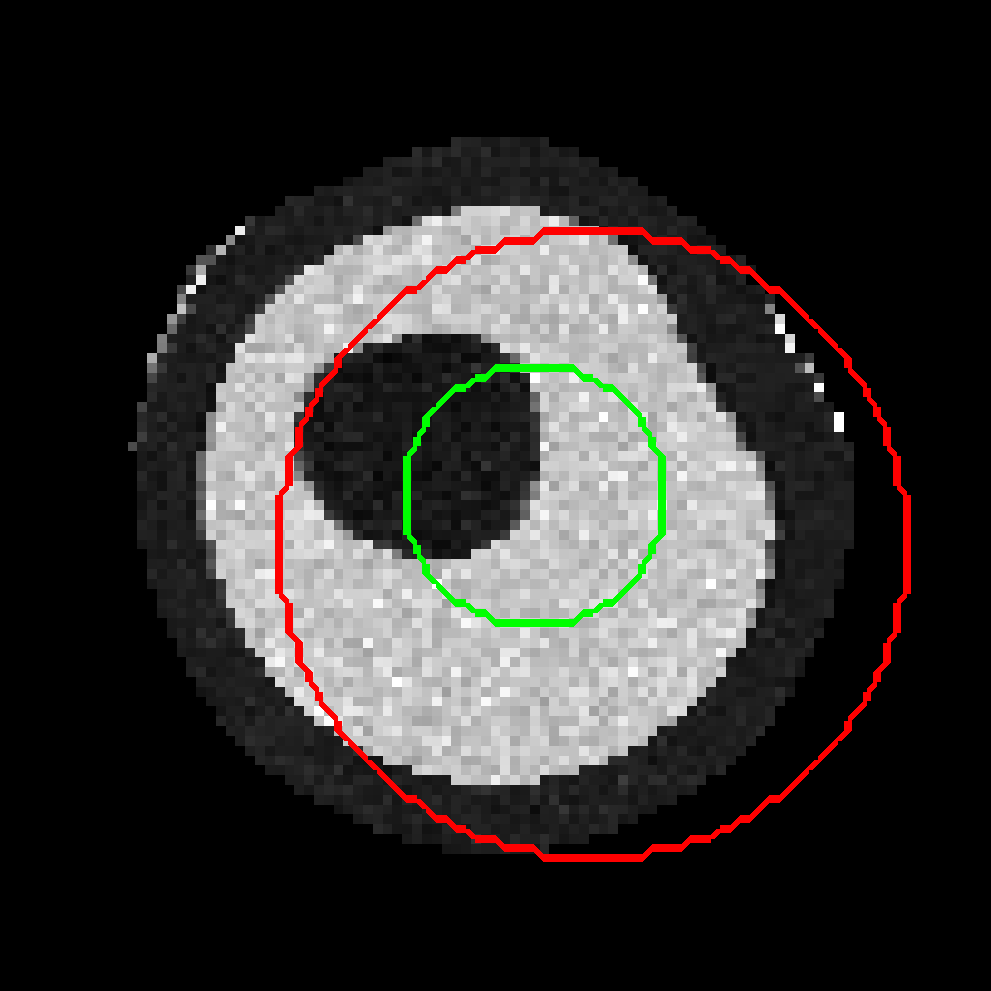
\includegraphics[width=0.19\textwidth]{model1result_b_2} &
%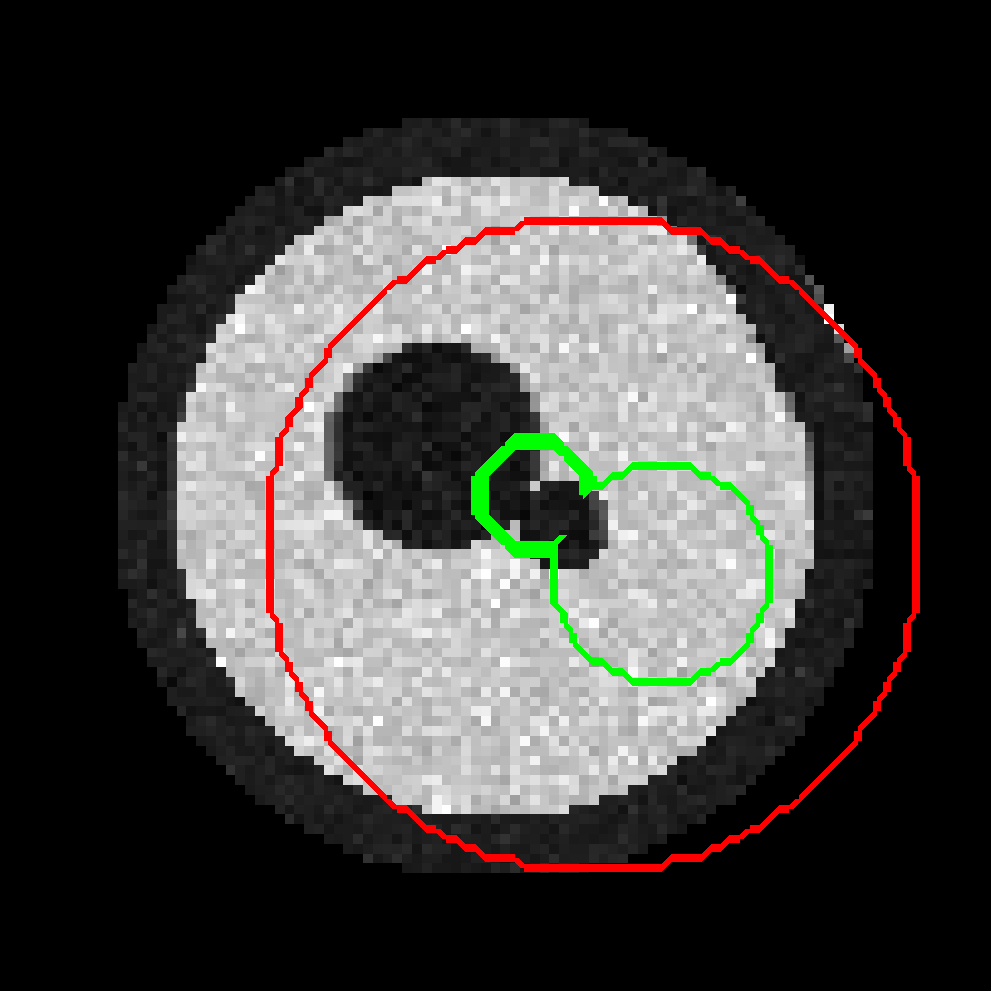
\includegraphics[width=0.19\textwidth]{model1result_b_3} &
%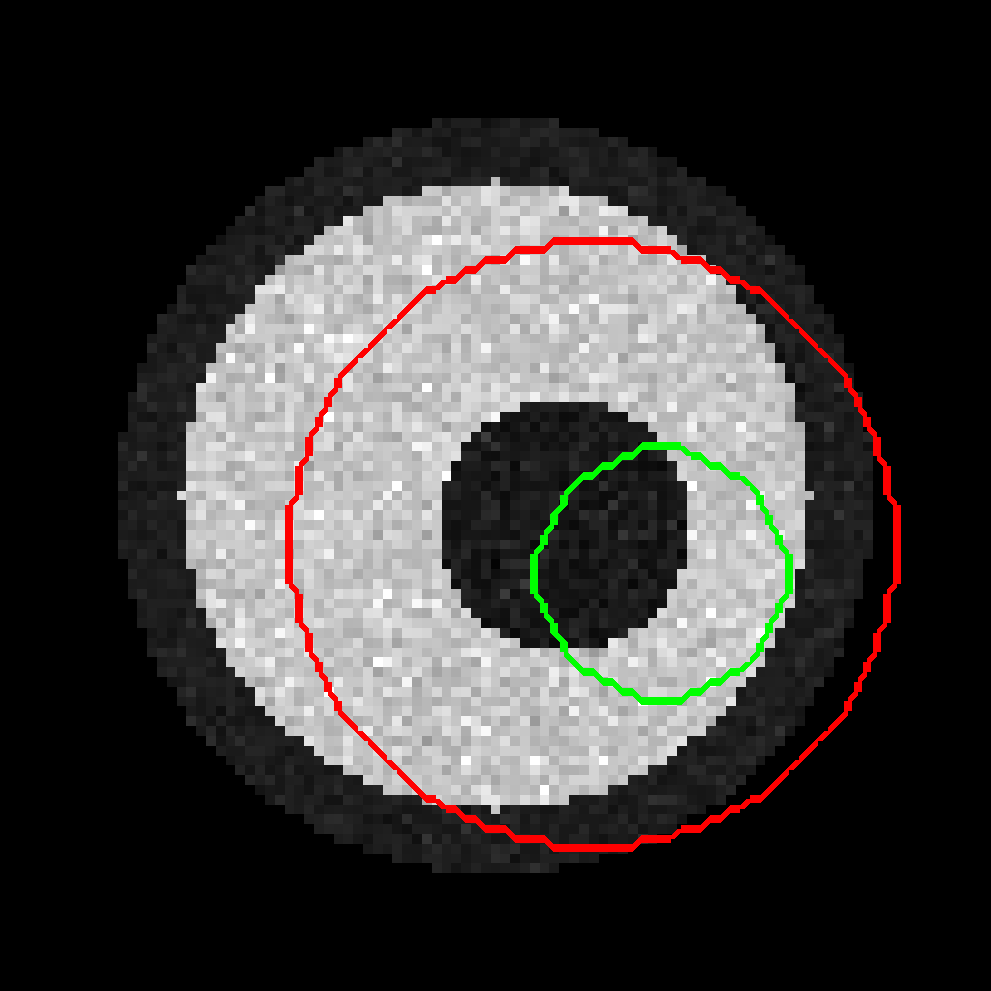
\includegraphics[width=0.19\textwidth]{model1result_b_4} &
%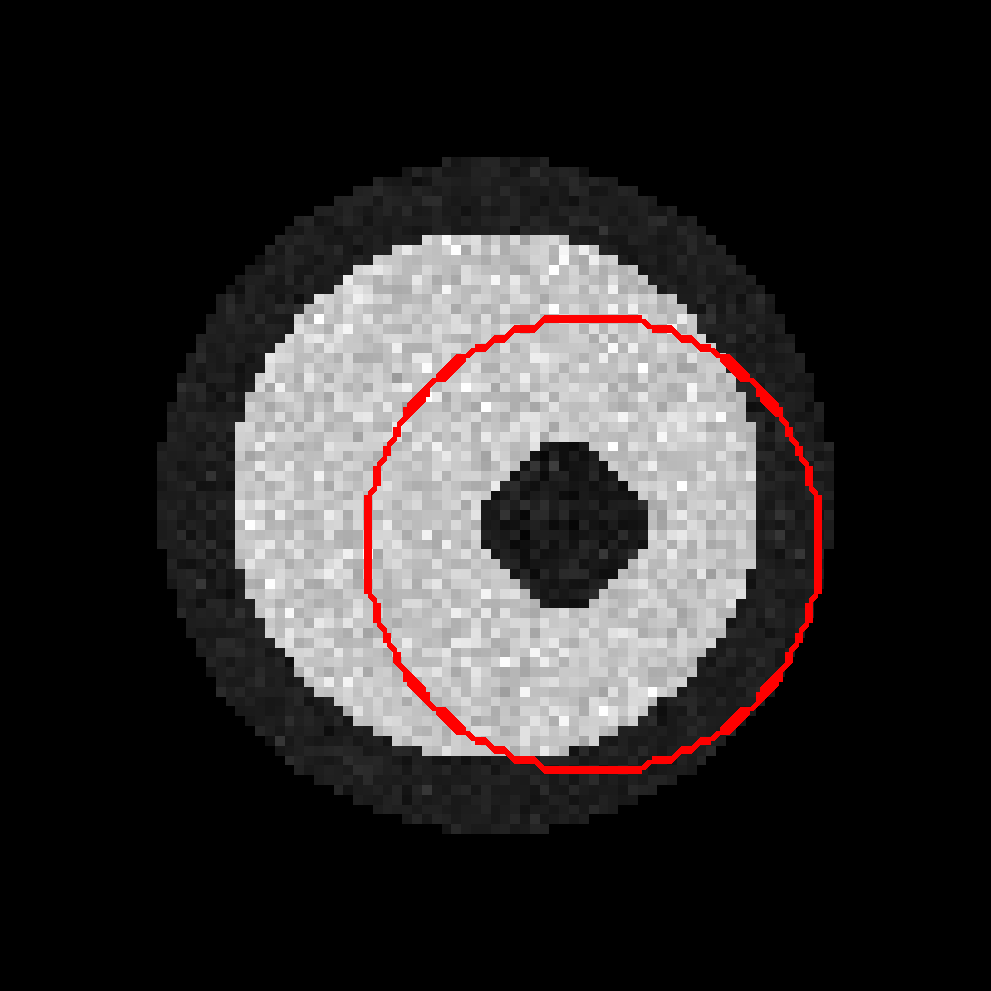
\includegraphics[width=0.19\textwidth]{model1result_b_5} \\
%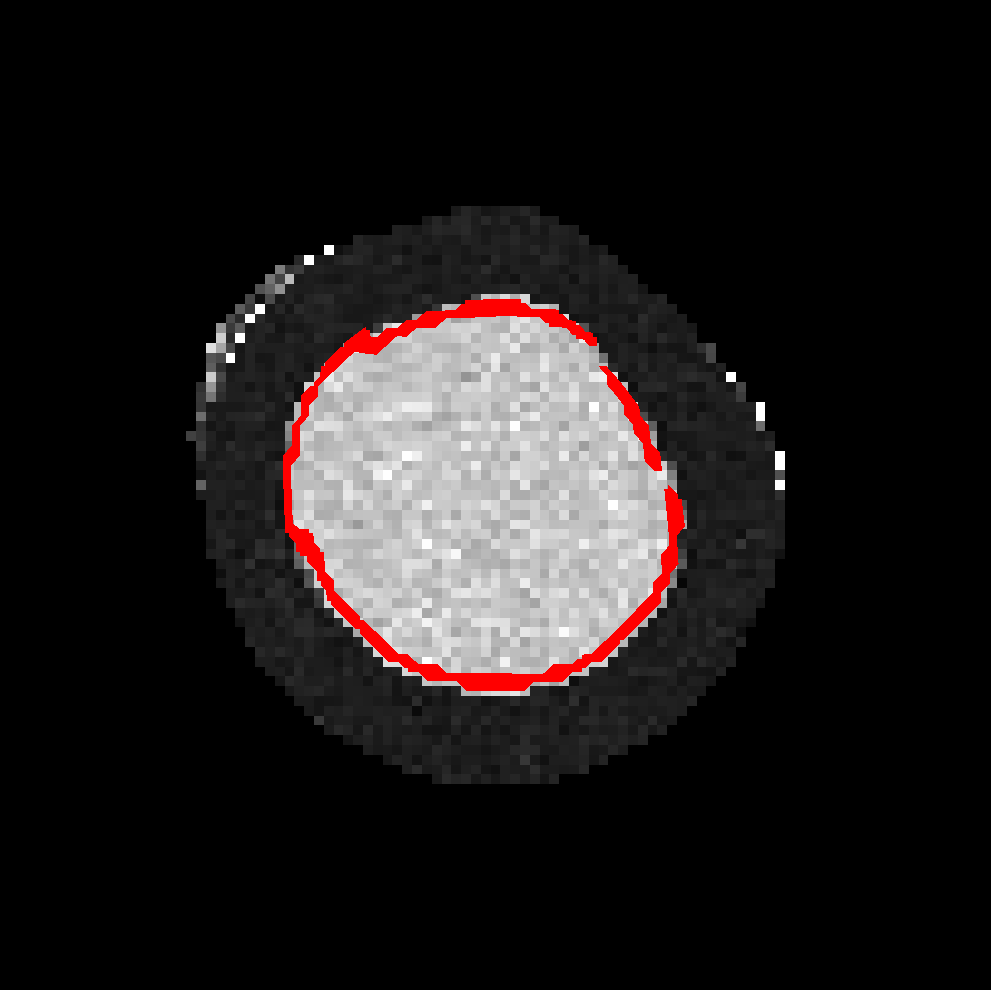
\includegraphics[width=0.19\textwidth]{IPMI2013-011} &
%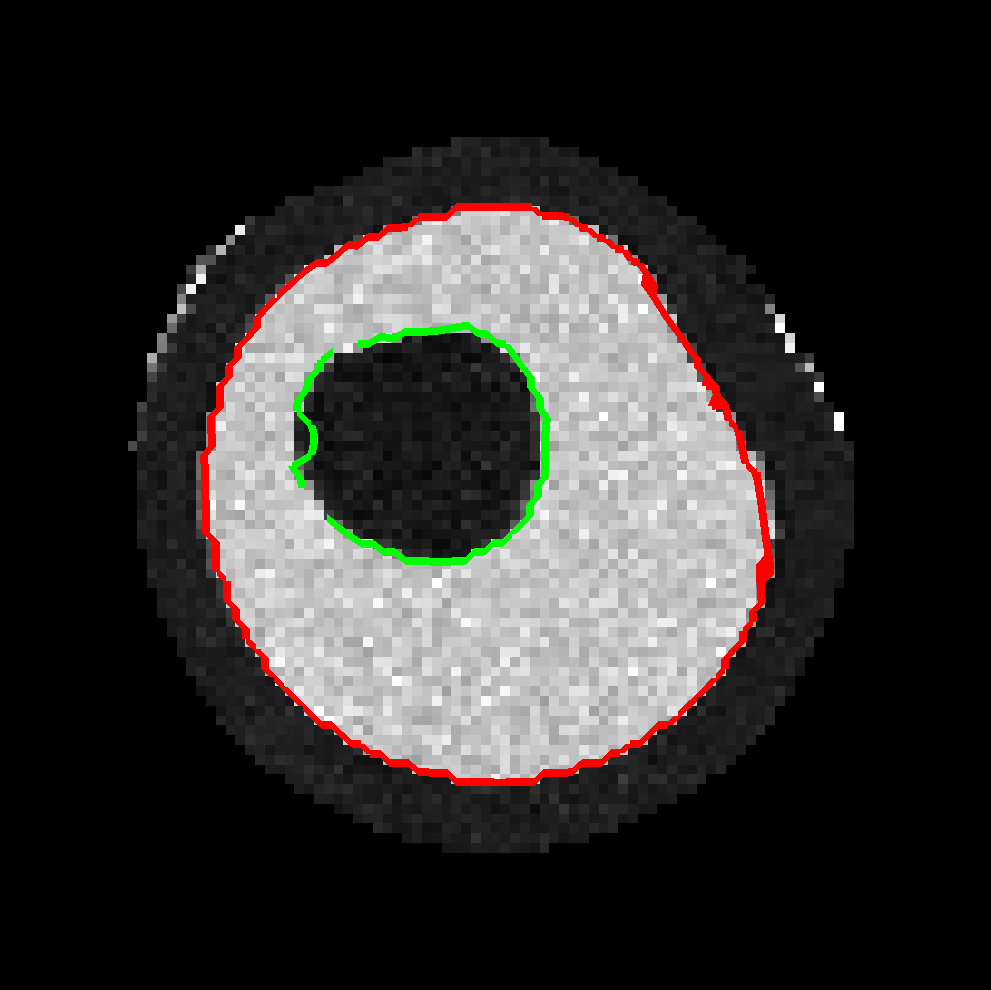
\includegraphics[width=0.19\textwidth]{IPMI2013-012} &
%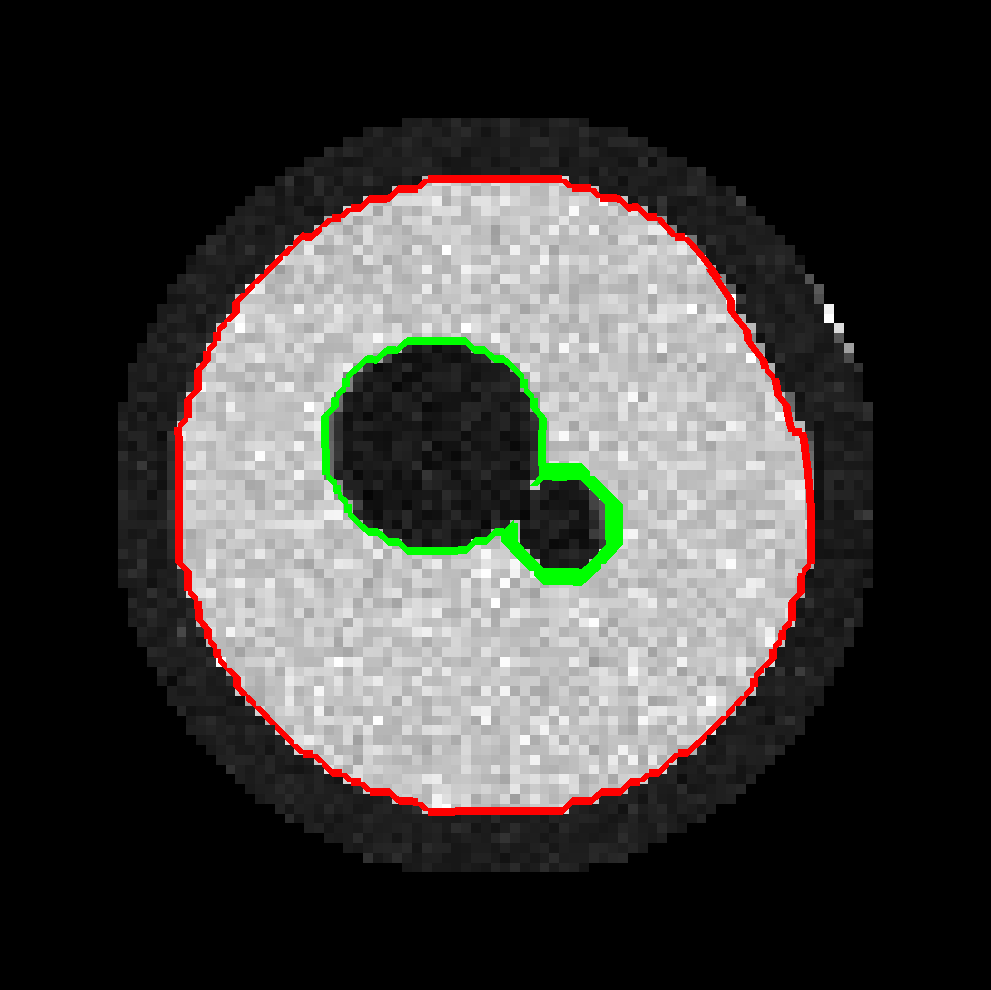
\includegraphics[width=0.19\textwidth]{IPMI2013-013} &
%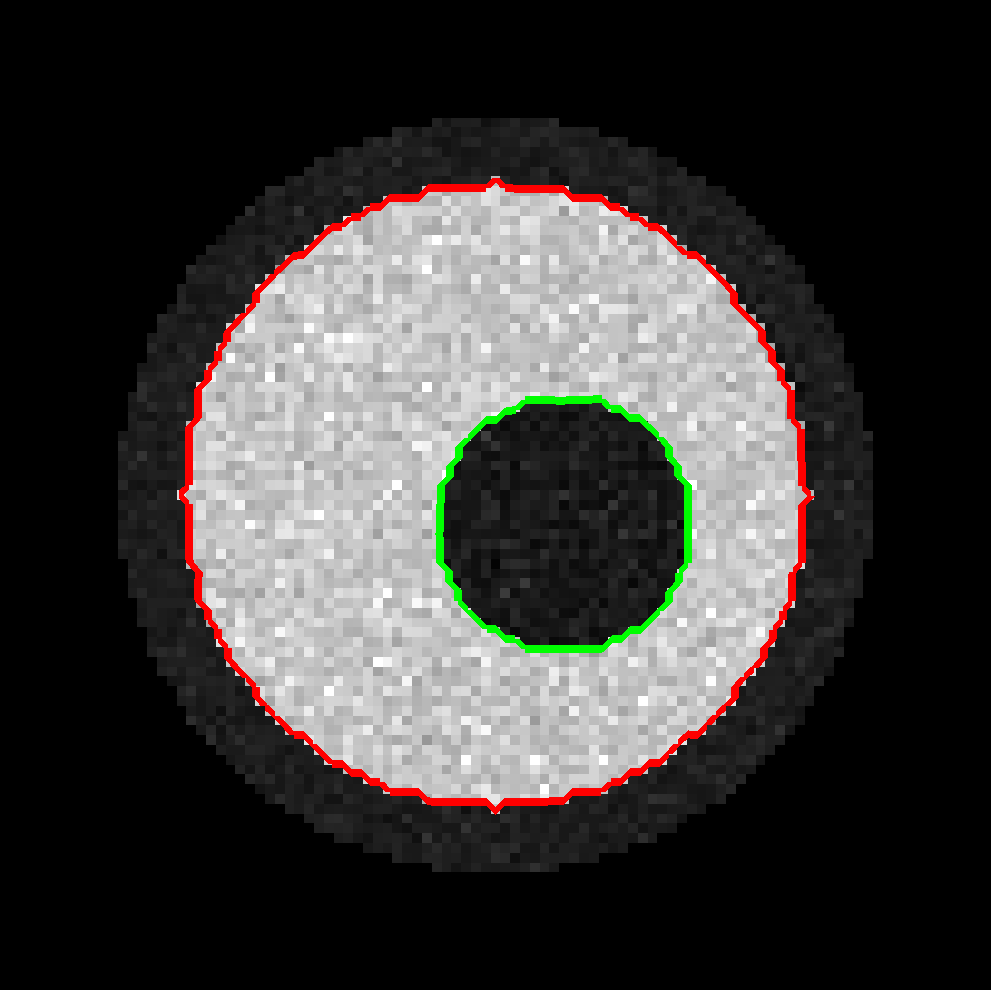
\includegraphics[width=0.19\textwidth]{IPMI2013-014} &
%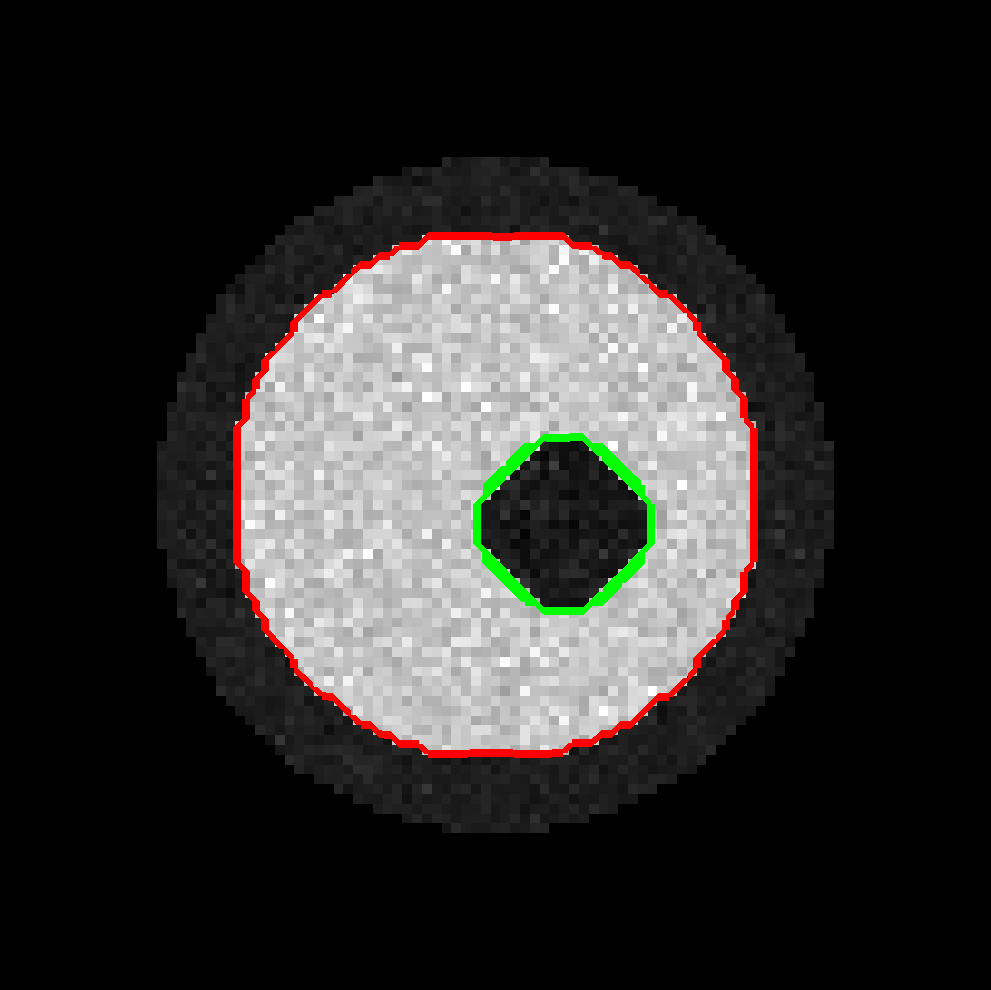
\includegraphics[width=0.19\textwidth]{IPMI2013-015} \\
%%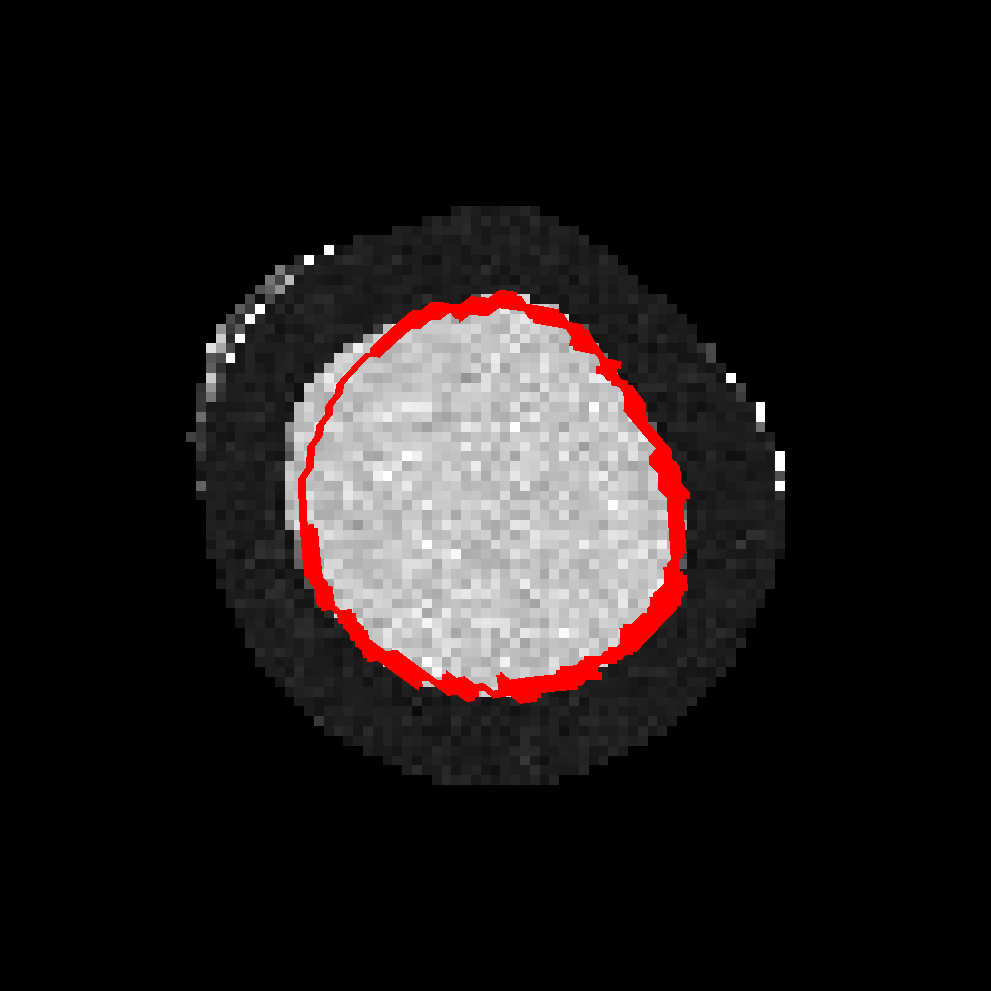
\includegraphics[width=0.19\textwidth]{model1result_a_1} &
%%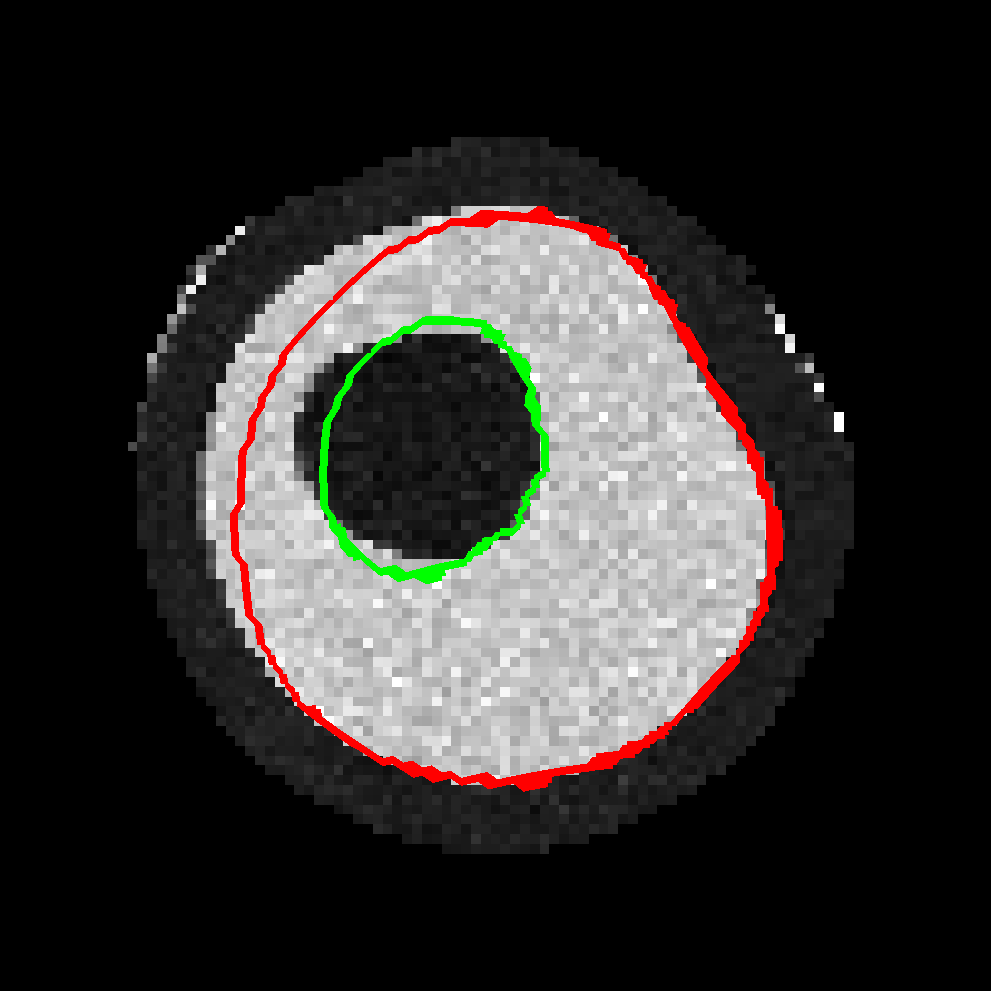
\includegraphics[width=0.19\textwidth]{model1result_a_2} &
%%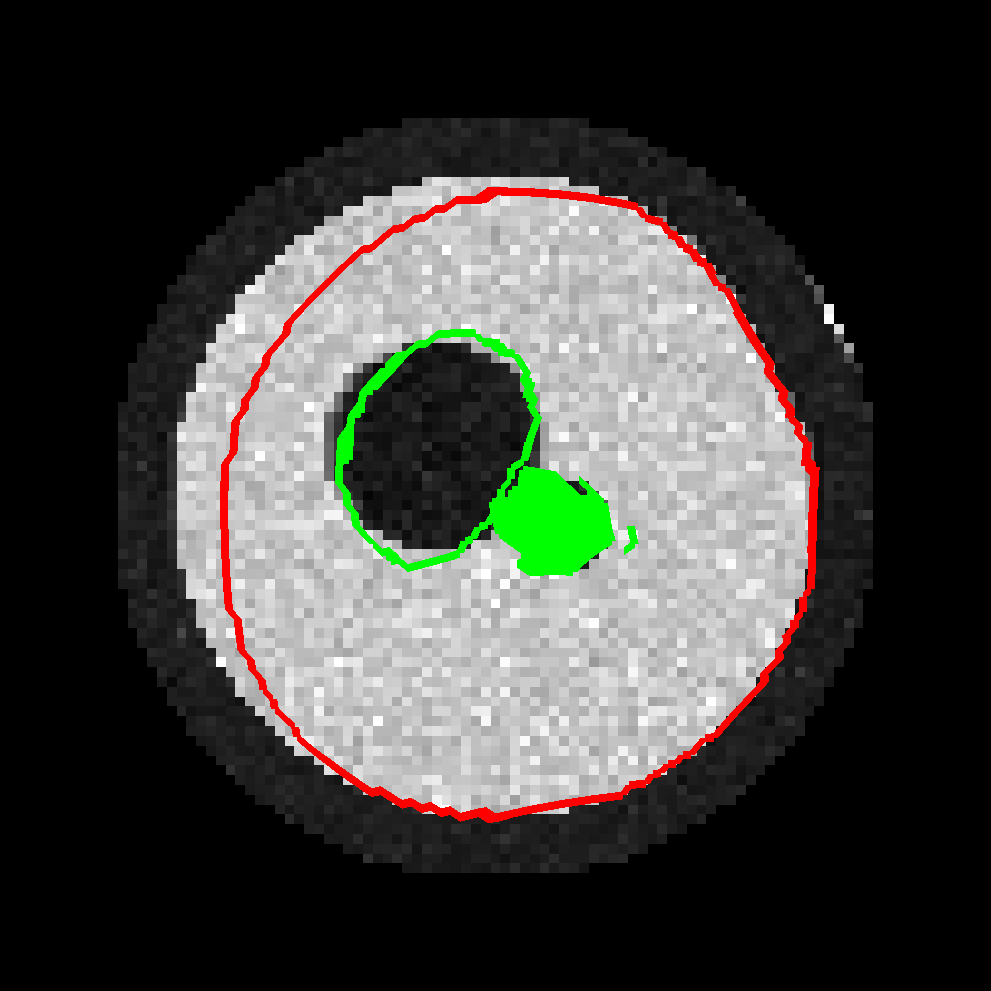
\includegraphics[width=0.19\textwidth]{model1result_a_3} &
%%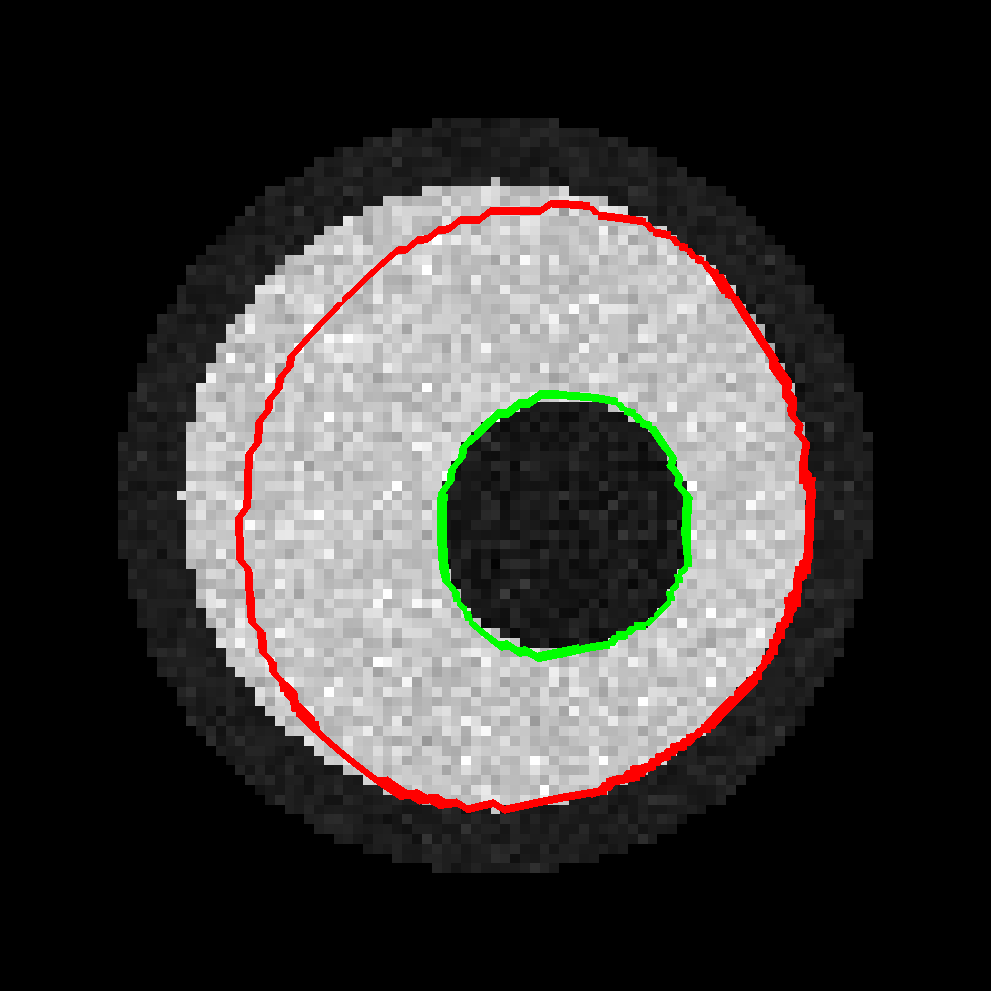
\includegraphics[width=0.19\textwidth]{model1result_a_4} &
%%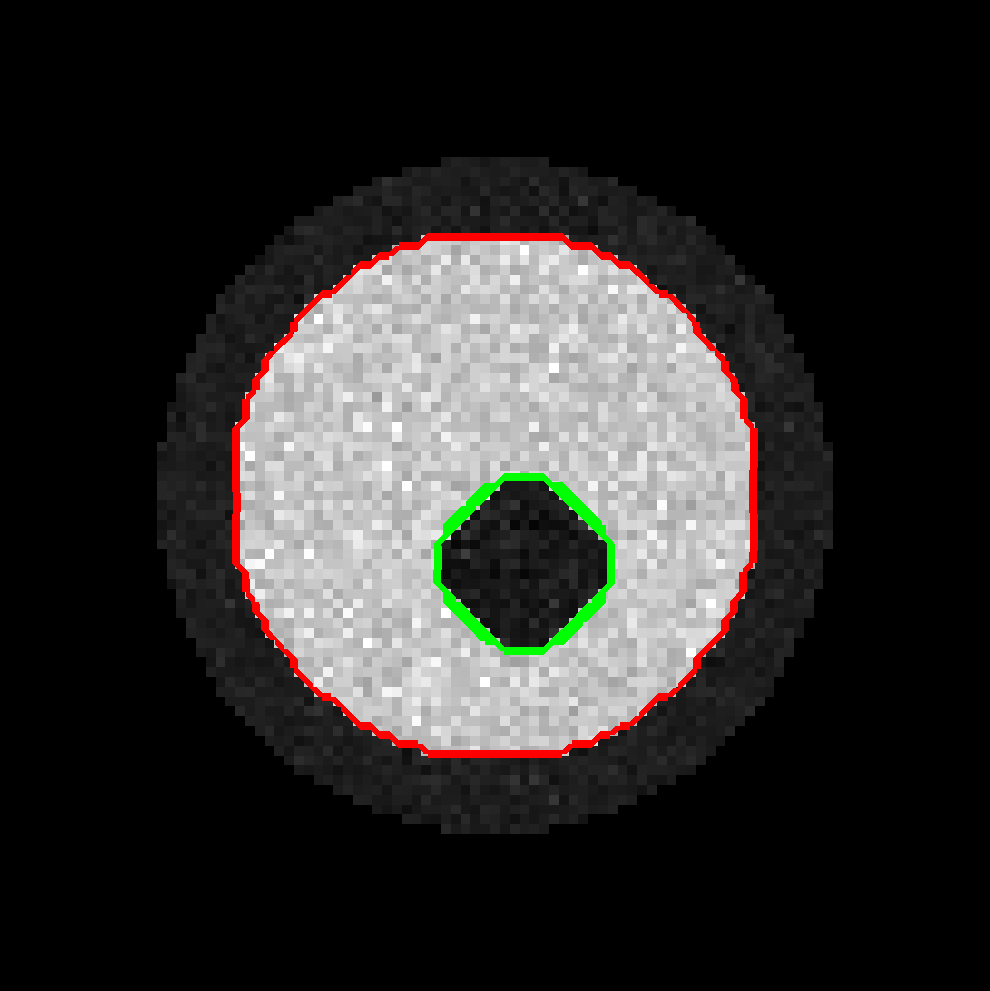
\includegraphics[width=0.19\textwidth]{model1result_a_5} \\
%\end{tabular}
%\caption{First row presents several slices along Z axis of the distorted \gls{fa} map and
%the undistorted \gls{wm}-\gls{gm} and \gls{wm}-\gls{csf} contours given as shape priors,
%subjected to the shift of [5.0,10.0,-5.0] mm. described in \autoref{sec:simulated_dwi}.
%Second row contains the same map, now with the contours after joint segmentation-registration.}
%\label{fig:fa}
%\end{figure}


% An example of a floating figure using the graphicx package.
% Note that \label must occur AFTER (or within) \caption.
% For figures, \caption should occur after the \includegraphics.
% Note that IEEEtran v1.7 and later has special internal code that
% is designed to preserve the operation of \label within \caption
% even when the captionsoff option is in effect. However, because
% of issues like this, it may be the safest practice to put all your
% \label just after \caption rather than within \caption{}.
%
% Reminder: the "draftcls" or "draftclsnofoot", not "draft", class
% option should be used if it is desired that the figures are to be
% displayed while in draft mode.
%
%\begin{figure}[!t]
%\centering
%\includegraphics[width=2.5in]{myfigure}
% where an .eps filename suffix will be assumed under latex,
% and a .pdf suffix will be assumed for pdflatex; or what has been declared
% via \DeclareGraphicsExtensions.
%\caption{Simulation Results.}
%\label{fig_sim}
%\end{figure}

% Note that IEEE typically puts floats only at the top, even when this
% results in a large percentage of a column being occupied by floats.


% An example of a double column floating figure using two subfigures.
% (The subfig.sty package must be loaded for this to work.)
% The subfigure \label commands are set within each subfloat command,
% and the \label for the overall figure must come after \caption.
% \hfil is used as a separator to get equal spacing.
% Watch out that the combined width of all the subfigures on a
% line do not exceed the text width or a line break will occur.
%
%\begin{figure*}[!t]
%\centering
%\subfloat[Case I]{\includegraphics[width=2.5in]{box}%
%\label{fig_first_case}}
%\hfil
%\subfloat[Case II]{\includegraphics[width=2.5in]{box}%
%\label{fig_second_case}}
%\caption{Simulation results.}
%\label{fig_sim}
%\end{figure*}
%
% Note that often IEEE papers with subfigures do not employ subfigure
% captions (using the optional argument to \subfloat[]), but instead will
% reference/describe all of them (a), (b), etc., within the main caption.


% An example of a floating table. Note that, for IEEE style tables, the
% \caption command should come BEFORE the table. Table text will default to
% \footnotesize as IEEE normally uses this smaller font for tables.
% The \label must come after \caption as always.
%
%\begin{table}[!t]
%% increase table row spacing, adjust to taste
%\renewcommand{\arraystretch}{1.3}
% if using array.sty, it might be a good idea to tweak the value of
% \extrarowheight as needed to properly center the text within the cells
%\caption{An Example of a Table}
%\label{table_example}
%\centering
%% Some packages, such as MDW tools, offer better commands for making tables
%% than the plain LaTeX2e tabular which is used here.
%\begin{tabular}{|c||c|}
%\hline
%One & Two\\
%\hline
%Three & Four\\
%\hline
%\end{tabular}
%\end{table}


% Note that IEEE does not put floats in the very first column - or typically
% anywhere on the first page for that matter. Also, in-text middle ("here")
% positioning is not used. Most IEEE journals use top floats exclusively.
% Note that, LaTeX2e, unlike IEEE journals, places footnotes above bottom
% floats. This can be corrected via the \fnbelowfloat command of the
% stfloats package.

% -*- root: 00-main.tex -*-
\section*{Conclusion}
\label{sec:regseg-conclusion}

\Regseg{} is a variational framework for the simultaneous segmentation and
  registration of 3D \gls*{dmri} data obtained from the human brain, where within-subject
  anatomical information is used as a reference.
The registration method segments the target multivariate image into several competing regions, which are
  defined explicitly by their limiting surfaces.
The surfaces are active and they evolve on a free-form deformation field supported by the B-spline basis.
A descent optimization strategy is guided by shape gradients computed on the current partition
  of the target image.
\Regseg{} uses active contours without edges and it searches for
  homogeneous regions within the image.
We tested \regseg{} using digital phantoms by simulating \gls*{t1} and \gls*{t2} \gls*{mri}
  warped with smooth random deformations.
The resulting misregistration of the contours was significantly lower than the image resolution
  of the phantoms.

We proposed \regseg{} for simultaneously segmenting and registering \gls*{dmri} data to
  their corresponding \gls*{t1} image from the same subject.
We demonstrated the accuracy of the proposed method based on visual assessments of the results
  obtained by \regseg{} and cross-comparisons with a widely used technique.
Moreover, \regseg{} does not require any images in addition to the minimal acquisition protocol,
  which only utilizes \gls*{t1} and \gls*{dmri}.
As well as the proposed application to \gls*{dmri} data, other potential uses of \regseg{} are
  atlas-based segmentation and tracking objects in time-series.


\section*{Availability and reproducibility statement}
\label{sec:regseg-availability}
We considered the reproducibility of our results as a design requirement.
Therefore, we used real data obtained from the Human Connectome Project \citep{essen_human_2012}
  and all of the software utilized in this study is also publicly available.
\Regseg{} was implemented on top of ITK-4.6 (Insight Registration and
  Segmentation Toolkit, \url{http://www.itk.org}).
The evaluation instruments (\autoref{fig:regseg-evworkflows}) were implemented using
  \emph{nipype} \citep{gorgolewski_nipype_2011} to assess their reproducibility.
All of the research elements (data, source code, figures, manuscript sources, etc.) involved in this study
  are publicly available under a unique package \citep{esteban_regseg_2015}.



% Add appendices
%% if have a single appendix:
%\appendix[Proof of the Zonklar Equations]
% or
%\appendix  % for no appendix heading
% do not use \section anymore after \appendix, only \section*
% is possibly needed

% use appendices with more than one appendix
% then use \section to start each appendix
% you must declare a \section before using any
% \subsection or using \label (\appendices by itself
% starts a section numbered zero.)
%
\onecolumn
\appendix

\section{Proof of duality between the probabilistic and the presented frameworks}
Here the demonstration that we are preparing.

% you can choose not to have a title for an appendix
% if you want by leaving the argument blank
%\section{}
%Appendix two text goes here.

In the probabilistic approach to image segmentation, the smoothness constraints
can be introduced into the \gls{map} criterion as a \gls{mrf}. Accordingly to the
Hammersley-Clifford theorem (\textbf{FIXME}: citations needed), an \gls{mrf} can
be equivalently characterized by a Gibb's distribution:
\begin{equation}
P(\mathbf{K})=\underset{i}{\prod} Z(U)^{-1}\,e^{-U(\mathbf{x}_i \mid \beta,K)} = \mathit{const.}\,e^{- \sum\limits_i \left( U(\mathbf{x}_i \mid \beta,K) \right) } \sim e^{-\nu_B \left| K \right| }.
\end{equation}
This way, we include the assumption that the total length of the edge set $K$ is small
and we draw the equivalence with the \gls{mrf} modeling, for $U(\mathbf{x}_i \mid \beta,K)$
being the Potts model.

In the probabilistic approach, the underlying concept to segmenting an image is the
Bayes' rule. For a discrete image of $N$ pixels indexed by $i$, this rule reads as
follows:
\begin{equation}
P(K|I)=P(I \mid K)\, P(K)=\underset{i}{\prod} p (\mathbf{x}_i | K ) \, p_i(K).
\end{equation}
The normalizer probability $P(I)$ has been omitted for simplicity.

In order to express the likelihood as an absolute energy in our variation framework,
the \textit{log}-likelihood is computed:
\begin{equation}
E(K)= -\log( P(K|I) ) = \sum\limits_k \int_{\Omega_k} -\log p_k(I(\mathbf{x}),\mathbf{x}) \,d\mathbf{x}+\nu_B \left|K\right|,
\end{equation}
where $\mathbf{s} = I(\mathbf{x})$, $\mathbf{s} \in \mathbb{R}^C$ (a vector of $C$ scalar features).
Additionally, the discrete grid of $N$ pixels has been converted to a continuous space by assuming
$d\mathbf{x}$ as infinitesimal bin size.

To explicitly define the likelihood, we firstly define the squared \textit{Mahalanobis distance} that
is the exponential of a multivariate normal distribution:
\begin{equation}
\Delta^2_k (\mathbf{s}) = (\mathbf{s} - \boldsymbol{\mu}_k)^T \, \Sigma^{-1}_k \, (\mathbf{s} - \boldsymbol{\mu}_k).
\end{equation}

Therefore, the likelihood is defined as follows:
\begin{equation}
p_k(I(\mathbf{x}),\mathbf{x}) = p_k(\mathbf{s},\mathbf{x})= p_k(\mathbf{s}) = \frac{1}{ \sqrt{(2\pi)^{C}\,\left|\boldsymbol{\Sigma}_{k}\right|}}\,{e^{\left(-\frac{1}{2}  \Delta^2_k (\mathbf{s}) \right)}}.
\end{equation}

Introducing this definition on (14), we have:
\begin{equation}
E(K)= \sum\limits_k \int_{\Omega_k} -\log{\left[ \frac{1}{ \sqrt{(2\pi)^{C}\,\left|\boldsymbol{\Sigma}_{k}\right|}}\,e^{\left(-\frac{1}{2}  \Delta^2_k (\mathbf{s}) \right)} \right] } \,d\mathbf{x}+\nu_B \left|K\right|.
\end{equation}

\begin{equation}
E(K) = \sum\limits_k \int_{\Omega_k} \left( \frac{1}{2} \log{ \left( (2\pi)^{C}\,\left|\boldsymbol{\Sigma}_{k}\right| \right)} + \frac{1}{2}  \Delta^2_k (\mathbf{s}) \right) \,d\mathbf{x}+\nu_B \left|K\right|
\end{equation}

\begin{equation}
E(K) = \sum\limits_k \left( \frac{ V_k }{2} \log{ \left( (2\pi)^{C}\,\left|\boldsymbol{\Sigma}_{k}\right| \right)}+ \frac{1}{2} \int_{\Omega_k} \Delta^2_k (\mathbf{s}) \,d\mathbf{x}+\nu_B \left|K\right| \right)
\end{equation}

{\color{red} {Using the region descriptors derived in \autoref{sec:regseg-methods_map}, we propose
an \gls{adf}-like, \gls{acwe}-based, piece-wise constant, image segmentation
model (where the unknown is the deformation field)
\cite{chan_active_2001} with the energy functional obtained in
\eqref{eq:regseg-final_map_energy}. This inverse problem is ill-posed
\cite{bertero_illposed_1988,hadamard_sur_1902}.
In order to account for deformation field regularity and to render the
problem well-posed, we include limiting and regularization terms into
the energy functional \cite{morozov_linear_1975,tichonov_solution_1963}:
%
\begin{multline}
E(u) = \sum\limits_l \int_{\Omega'_l} \mdist{f}{l} \,d\vec{x} \\
+ \int \vec{u}^T \, A \, \vec{u} \, d\vec{x} + \int \tr\{(\nabla \vec{u}^T)^T B (\nabla \vec{u}^T)\} d\vec{x}
\label{eq:regseg-complete_energy}
\end{multline}
%
These regularity terms ensure that the segmenting contours in
\gls{dwi} space are still close to their native shape. The model
easily allows to incorporate inhomogeneous and anisotropic
regularization \cite{nagel_investigation_1986} to better regularize
the \gls{epi} distortion.}}

\todo[inline]{this last paragraphs in red color were located a bit
further, but I think we can keep some of the refs and still reproduce
the continuous version of the energy functional}

\section{Extensions}

\subsubsection{Semi-implicit Euler-forward optimization}
It is necessary to discretize $t$ in order to obtain a numerical
implementation of the equation \eqref{eq:regseg-gradient_final}:
\begin{align}
\frac{\vec{u}_k^{t+1}-\vec{u}_k^t}{\tau} =
&- \underset{l,m}{\sum} \underset{i}{\sum}
\left[ \mdist{f_i'}{l} - \mdist{f_i'}{m}\right]
\psi_k(\vec{c}_i)\, \hat{\vec{n}}_i \notag\\
&+2\, \boldsymbol{\alpha} \vec{u}_k^{t+1}
-2\, \boldsymbol{\beta} \Delta \vec{u}_k^{t+1}.
\end{align}

The associated Euler-Lagrange equation is found as:
\begin{equation}
(\tau^{-1} +2\, \boldsymbol{\alpha} - 2\, \boldsymbol{\beta} \Delta )\, \vec{u}_k^{t+1} =
\tau^{-1} \vec{u}_k^t - \frac{\partial}{\partial \vec{u}_k} E_{data}(\vec{u}_k^t),
\end{equation}
that is a linear system that we translate into Fourier domain,
to obtain the next deformation field $\vec{u}_k^{t+1}$:
\begin{multline}
\vec{u}_k^{t+1} = \\
 \mathcal{F}^{-1} \left\lbrace
\frac{\mathcal{F}\lbrace \tau^{-1}\vec{u}_{k}^{t} - \underset{l,m}{\sum} \underset{i}{\sum}
\left[ \mdist{f_i'}{l} - \mdist{f_i'}{m}\right] \rbrace}
     {\mathcal{F}\lbrace (\tau^{-1} +2\,\boldsymbol{\alpha})\mathcal{I} - 2\,\boldsymbol{\beta} \Delta ) \rbrace}
     \right\rbrace
\end{multline}

Here, we rewrite the Laplacian as a linear combination of the identity and shift operators:
\begin{equation}
\Delta = \sum\limits_d \mathcal{S}_d^- + \mathcal{S}_d^+ - 2 \mathcal{I}
\end{equation}
where $\mathcal{S}_{d}^{\pm}$ stands for the forward ($+$) and backward ($-$) shift
operator along coordinates axis $d$, of which the Fourier transform is found easily as
\begin{equation}
\mathcal{F}\{\mathcal{S}_{d}^{\pm}\} = e^{\pm \vec{i}\omega_{d}},
\end{equation}
where $\omega_{d}$ is the normalized pulsation along $d$-direction. Accordingly, the
Fourier transform of the discrete Laplacian is found as
\begin{equation}
\mathcal{F}\{\Delta\} = \sum\limits_d e^{-\vec{i}\omega_d } + e^{\vec{i}\omega_d } - 2 = \sum\limits_d \left( 2\cos(\omega_d) - 2 \right)
\end{equation}

The remaining transforms are trivial or can be computed using the \gls{fft}
as in \citep{estellers_efficient_2011}.

% ACKs
% -*- root: 00-main.tex -*-
% use section* for acknowledgement
\section*{Author contributions}
OE implemented the method, designed and conducted the experiments, wrote the paper,
  simulated the phantoms and prepared the real data.
DZ devised and drafted the registration method, generated early phantom datasets and
  collaborated with the implementation of the method.
AD, MBC and MJLC interpreted the results.
AD, MBC, MJLC, JPT and AS advised on all aspects of the work.
All the authors contributed in editing the paper.

\section*{Acknowledgment}
The authors thank V. Estellers for early discussions at the beginning of this project,
  and L. Vese for her support during OE's research visits in her laboratory.

This study is supported by: the Spain's Ministry of Science and Innovation
  (projects TEC2010-21619- C04-03, TEC2011-28972-C02-02, CDTI-CENIT
  AMIT and INNPACTO PRECISION), Comunidad de Madrid (ARTEMIS) and
  European Regional Development Funds; the Center for Biomedical Imaging
  (CIBM) of the Geneva and Lausanne Universities and the EPFL, as well as the
  Leenaards and Louis Jeantet foundations.
DZ is supported by the Swiss National Science Foundation (SNF) under grant PBELP2-137727.



% Can use something like this to put references on a page
% by themselves when using endfloat and the captionsoff option.
\ifCLASSOPTIONcaptionsoff
  \newpage
\fi



% trigger a \newpage just before the given reference
% number - used to balance the columns on the last page
% adjust value as needed - may need to be readjusted if
% the document is modified later
%\IEEEtriggeratref{8}
% The "triggered" command can be changed if desired:
%\IEEEtriggercmd{\enlargethispage{-5in}}

% references section

% can use a bibliography generated by BibTeX as a .bbl file
% BibTeX documentation can be easily obtained at:
% http://www.ctan.org/tex-archive/biblio/bibtex/contrib/doc/
% The IEEEtran BibTeX style support page is at:
% http://www.michaelshell.org/tex/ieeetran/bibtex/
%\bibliographystyle{IEEEtran}
\bibliographystyle{myplainnat}
% argument is your BibTeX string definitions and bibliography database(s)
\bibliography{Remote}

% biography section
%
% If you have an EPS/PDF photo (graphicx package needed) extra braces are
% needed around the contents of the optional argument to biography to prevent
% the LaTeX parser from getting confused when it sees the complicated
% \includegraphics command within an optional argument. (You could create
% your own custom macro containing the \includegraphics command to make things
% simpler here.)
%\begin{IEEEbiography}[{\includegraphics[width=1in,height=1.25in,clip,keepaspectratio]{mshell}}]{Michael Shell}
% or if you just want to reserve a space for a photo:
%\begin{IEEEbiography}{Oscar Esteban}
%Biography text here.
%\end{IEEEbiography}
% if you will not have a photo at all:
%\begin{IEEEbiographynophoto}{John Doe}
%Biography text here.
%\end{IEEEbiographynophoto}

% insert where needed to balance the two columns on the last page with
% biographies
%\newpage

%\begin{IEEEbiographynophoto}{Jane Doe}
%Biography text here.
%\end{IEEEbiographynophoto}

% You can push biographies down or up by placing
% a \vfill before or after them. The appropriate
% use of \vfill depends on what kind of text is
% on the last page and whether or not the columns
% are being equalized.
%\vfill
% Can be used to pull up biographies so that the bottom of the last one
% is flush with the other column.
%\enlargethispage{-5in}

% that's all folks
\end{document}


